\documentclass[11pt]{article}

    \usepackage[breakable]{tcolorbox}
    \usepackage{parskip} % Stop auto-indenting (to mimic markdown behaviour)
    
    \usepackage{iftex}
    \ifPDFTeX
    	\usepackage[T1]{fontenc}
    	\usepackage{mathpazo}
    \else
    	\usepackage{fontspec}
    \fi

    % Basic figure setup, for now with no caption control since it's done
    % automatically by Pandoc (which extracts ![](path) syntax from Markdown).
    \usepackage{graphicx}
    % Maintain compatibility with old templates. Remove in nbconvert 6.0
    \let\Oldincludegraphics\includegraphics
    % Ensure that by default, figures have no caption (until we provide a
    % proper Figure object with a Caption API and a way to capture that
    % in the conversion process - todo).
    \usepackage{caption}
    \DeclareCaptionFormat{nocaption}{}
    \captionsetup{format=nocaption,aboveskip=0pt,belowskip=0pt}

    \usepackage{float}
    \floatplacement{figure}{H} % forces figures to be placed at the correct location
    \usepackage{xcolor} % Allow colors to be defined
    \usepackage{enumerate} % Needed for markdown enumerations to work
    \usepackage{geometry} % Used to adjust the document margins
    \usepackage{amsmath} % Equations
    \usepackage{amssymb} % Equations
    \usepackage{textcomp} % defines textquotesingle
    % Hack from http://tex.stackexchange.com/a/47451/13684:
    \AtBeginDocument{%
        \def\PYZsq{\textquotesingle}% Upright quotes in Pygmentized code
    }
    \usepackage{upquote} % Upright quotes for verbatim code
    \usepackage{eurosym} % defines \euro
    \usepackage[mathletters]{ucs} % Extended unicode (utf-8) support
    \usepackage{fancyvrb} % verbatim replacement that allows latex
    \usepackage{grffile} % extends the file name processing of package graphics 
                         % to support a larger range
    \makeatletter % fix for old versions of grffile with XeLaTeX
    \@ifpackagelater{grffile}{2019/11/01}
    {
      % Do nothing on new versions
    }
    {
      \def\Gread@@xetex#1{%
        \IfFileExists{"\Gin@base".bb}%
        {\Gread@eps{\Gin@base.bb}}%
        {\Gread@@xetex@aux#1}%
      }
    }
    \makeatother
    \usepackage[Export]{adjustbox} % Used to constrain images to a maximum size
    \adjustboxset{max size={0.9\linewidth}{0.9\paperheight}}

    % The hyperref package gives us a pdf with properly built
    % internal navigation ('pdf bookmarks' for the table of contents,
    % internal cross-reference links, web links for URLs, etc.)
    \usepackage{hyperref}
    % The default LaTeX title has an obnoxious amount of whitespace. By default,
    % titling removes some of it. It also provides customization options.
    \usepackage{titling}
    \usepackage{longtable} % longtable support required by pandoc >1.10
    \usepackage{booktabs}  % table support for pandoc > 1.12.2
    \usepackage[inline]{enumitem} % IRkernel/repr support (it uses the enumerate* environment)
    \usepackage[normalem]{ulem} % ulem is needed to support strikethroughs (\sout)
                                % normalem makes italics be italics, not underlines
    \usepackage{mathrsfs}
    

    
    % Colors for the hyperref package
    \definecolor{urlcolor}{rgb}{0,.145,.698}
    \definecolor{linkcolor}{rgb}{.71,0.21,0.01}
    \definecolor{citecolor}{rgb}{.12,.54,.11}

    % ANSI colors
    \definecolor{ansi-black}{HTML}{3E424D}
    \definecolor{ansi-black-intense}{HTML}{282C36}
    \definecolor{ansi-red}{HTML}{E75C58}
    \definecolor{ansi-red-intense}{HTML}{B22B31}
    \definecolor{ansi-green}{HTML}{00A250}
    \definecolor{ansi-green-intense}{HTML}{007427}
    \definecolor{ansi-yellow}{HTML}{DDB62B}
    \definecolor{ansi-yellow-intense}{HTML}{B27D12}
    \definecolor{ansi-blue}{HTML}{208FFB}
    \definecolor{ansi-blue-intense}{HTML}{0065CA}
    \definecolor{ansi-magenta}{HTML}{D160C4}
    \definecolor{ansi-magenta-intense}{HTML}{A03196}
    \definecolor{ansi-cyan}{HTML}{60C6C8}
    \definecolor{ansi-cyan-intense}{HTML}{258F8F}
    \definecolor{ansi-white}{HTML}{C5C1B4}
    \definecolor{ansi-white-intense}{HTML}{A1A6B2}
    \definecolor{ansi-default-inverse-fg}{HTML}{FFFFFF}
    \definecolor{ansi-default-inverse-bg}{HTML}{000000}

    % common color for the border for error outputs.
    \definecolor{outerrorbackground}{HTML}{FFDFDF}

    % commands and environments needed by pandoc snippets
    % extracted from the output of `pandoc -s`
    \providecommand{\tightlist}{%
      \setlength{\itemsep}{0pt}\setlength{\parskip}{0pt}}
    \DefineVerbatimEnvironment{Highlighting}{Verbatim}{commandchars=\\\{\}}
    % Add ',fontsize=\small' for more characters per line
    \newenvironment{Shaded}{}{}
    \newcommand{\KeywordTok}[1]{\textcolor[rgb]{0.00,0.44,0.13}{\textbf{{#1}}}}
    \newcommand{\DataTypeTok}[1]{\textcolor[rgb]{0.56,0.13,0.00}{{#1}}}
    \newcommand{\DecValTok}[1]{\textcolor[rgb]{0.25,0.63,0.44}{{#1}}}
    \newcommand{\BaseNTok}[1]{\textcolor[rgb]{0.25,0.63,0.44}{{#1}}}
    \newcommand{\FloatTok}[1]{\textcolor[rgb]{0.25,0.63,0.44}{{#1}}}
    \newcommand{\CharTok}[1]{\textcolor[rgb]{0.25,0.44,0.63}{{#1}}}
    \newcommand{\StringTok}[1]{\textcolor[rgb]{0.25,0.44,0.63}{{#1}}}
    \newcommand{\CommentTok}[1]{\textcolor[rgb]{0.38,0.63,0.69}{\textit{{#1}}}}
    \newcommand{\OtherTok}[1]{\textcolor[rgb]{0.00,0.44,0.13}{{#1}}}
    \newcommand{\AlertTok}[1]{\textcolor[rgb]{1.00,0.00,0.00}{\textbf{{#1}}}}
    \newcommand{\FunctionTok}[1]{\textcolor[rgb]{0.02,0.16,0.49}{{#1}}}
    \newcommand{\RegionMarkerTok}[1]{{#1}}
    \newcommand{\ErrorTok}[1]{\textcolor[rgb]{1.00,0.00,0.00}{\textbf{{#1}}}}
    \newcommand{\NormalTok}[1]{{#1}}
    
    % Additional commands for more recent versions of Pandoc
    \newcommand{\ConstantTok}[1]{\textcolor[rgb]{0.53,0.00,0.00}{{#1}}}
    \newcommand{\SpecialCharTok}[1]{\textcolor[rgb]{0.25,0.44,0.63}{{#1}}}
    \newcommand{\VerbatimStringTok}[1]{\textcolor[rgb]{0.25,0.44,0.63}{{#1}}}
    \newcommand{\SpecialStringTok}[1]{\textcolor[rgb]{0.73,0.40,0.53}{{#1}}}
    \newcommand{\ImportTok}[1]{{#1}}
    \newcommand{\DocumentationTok}[1]{\textcolor[rgb]{0.73,0.13,0.13}{\textit{{#1}}}}
    \newcommand{\AnnotationTok}[1]{\textcolor[rgb]{0.38,0.63,0.69}{\textbf{\textit{{#1}}}}}
    \newcommand{\CommentVarTok}[1]{\textcolor[rgb]{0.38,0.63,0.69}{\textbf{\textit{{#1}}}}}
    \newcommand{\VariableTok}[1]{\textcolor[rgb]{0.10,0.09,0.49}{{#1}}}
    \newcommand{\ControlFlowTok}[1]{\textcolor[rgb]{0.00,0.44,0.13}{\textbf{{#1}}}}
    \newcommand{\OperatorTok}[1]{\textcolor[rgb]{0.40,0.40,0.40}{{#1}}}
    \newcommand{\BuiltInTok}[1]{{#1}}
    \newcommand{\ExtensionTok}[1]{{#1}}
    \newcommand{\PreprocessorTok}[1]{\textcolor[rgb]{0.74,0.48,0.00}{{#1}}}
    \newcommand{\AttributeTok}[1]{\textcolor[rgb]{0.49,0.56,0.16}{{#1}}}
    \newcommand{\InformationTok}[1]{\textcolor[rgb]{0.38,0.63,0.69}{\textbf{\textit{{#1}}}}}
    \newcommand{\WarningTok}[1]{\textcolor[rgb]{0.38,0.63,0.69}{\textbf{\textit{{#1}}}}}
    
    
    % Define a nice break command that doesn't care if a line doesn't already
    % exist.
    \def\br{\hspace*{\fill} \\* }
    % Math Jax compatibility definitions
    \def\gt{>}
    \def\lt{<}
    \let\Oldtex\TeX
    \let\Oldlatex\LaTeX
    \renewcommand{\TeX}{\textrm{\Oldtex}}
    \renewcommand{\LaTeX}{\textrm{\Oldlatex}}
    % Document parameters
    % Document title
    \title{6.2 Building maps with the Extended Kalman Filter}
    
    
    
    
    
% Pygments definitions
\makeatletter
\def\PY@reset{\let\PY@it=\relax \let\PY@bf=\relax%
    \let\PY@ul=\relax \let\PY@tc=\relax%
    \let\PY@bc=\relax \let\PY@ff=\relax}
\def\PY@tok#1{\csname PY@tok@#1\endcsname}
\def\PY@toks#1+{\ifx\relax#1\empty\else%
    \PY@tok{#1}\expandafter\PY@toks\fi}
\def\PY@do#1{\PY@bc{\PY@tc{\PY@ul{%
    \PY@it{\PY@bf{\PY@ff{#1}}}}}}}
\def\PY#1#2{\PY@reset\PY@toks#1+\relax+\PY@do{#2}}

\expandafter\def\csname PY@tok@w\endcsname{\def\PY@tc##1{\textcolor[rgb]{0.73,0.73,0.73}{##1}}}
\expandafter\def\csname PY@tok@c\endcsname{\let\PY@it=\textit\def\PY@tc##1{\textcolor[rgb]{0.25,0.50,0.50}{##1}}}
\expandafter\def\csname PY@tok@cp\endcsname{\def\PY@tc##1{\textcolor[rgb]{0.74,0.48,0.00}{##1}}}
\expandafter\def\csname PY@tok@k\endcsname{\let\PY@bf=\textbf\def\PY@tc##1{\textcolor[rgb]{0.00,0.50,0.00}{##1}}}
\expandafter\def\csname PY@tok@kp\endcsname{\def\PY@tc##1{\textcolor[rgb]{0.00,0.50,0.00}{##1}}}
\expandafter\def\csname PY@tok@kt\endcsname{\def\PY@tc##1{\textcolor[rgb]{0.69,0.00,0.25}{##1}}}
\expandafter\def\csname PY@tok@o\endcsname{\def\PY@tc##1{\textcolor[rgb]{0.40,0.40,0.40}{##1}}}
\expandafter\def\csname PY@tok@ow\endcsname{\let\PY@bf=\textbf\def\PY@tc##1{\textcolor[rgb]{0.67,0.13,1.00}{##1}}}
\expandafter\def\csname PY@tok@nb\endcsname{\def\PY@tc##1{\textcolor[rgb]{0.00,0.50,0.00}{##1}}}
\expandafter\def\csname PY@tok@nf\endcsname{\def\PY@tc##1{\textcolor[rgb]{0.00,0.00,1.00}{##1}}}
\expandafter\def\csname PY@tok@nc\endcsname{\let\PY@bf=\textbf\def\PY@tc##1{\textcolor[rgb]{0.00,0.00,1.00}{##1}}}
\expandafter\def\csname PY@tok@nn\endcsname{\let\PY@bf=\textbf\def\PY@tc##1{\textcolor[rgb]{0.00,0.00,1.00}{##1}}}
\expandafter\def\csname PY@tok@ne\endcsname{\let\PY@bf=\textbf\def\PY@tc##1{\textcolor[rgb]{0.82,0.25,0.23}{##1}}}
\expandafter\def\csname PY@tok@nv\endcsname{\def\PY@tc##1{\textcolor[rgb]{0.10,0.09,0.49}{##1}}}
\expandafter\def\csname PY@tok@no\endcsname{\def\PY@tc##1{\textcolor[rgb]{0.53,0.00,0.00}{##1}}}
\expandafter\def\csname PY@tok@nl\endcsname{\def\PY@tc##1{\textcolor[rgb]{0.63,0.63,0.00}{##1}}}
\expandafter\def\csname PY@tok@ni\endcsname{\let\PY@bf=\textbf\def\PY@tc##1{\textcolor[rgb]{0.60,0.60,0.60}{##1}}}
\expandafter\def\csname PY@tok@na\endcsname{\def\PY@tc##1{\textcolor[rgb]{0.49,0.56,0.16}{##1}}}
\expandafter\def\csname PY@tok@nt\endcsname{\let\PY@bf=\textbf\def\PY@tc##1{\textcolor[rgb]{0.00,0.50,0.00}{##1}}}
\expandafter\def\csname PY@tok@nd\endcsname{\def\PY@tc##1{\textcolor[rgb]{0.67,0.13,1.00}{##1}}}
\expandafter\def\csname PY@tok@s\endcsname{\def\PY@tc##1{\textcolor[rgb]{0.73,0.13,0.13}{##1}}}
\expandafter\def\csname PY@tok@sd\endcsname{\let\PY@it=\textit\def\PY@tc##1{\textcolor[rgb]{0.73,0.13,0.13}{##1}}}
\expandafter\def\csname PY@tok@si\endcsname{\let\PY@bf=\textbf\def\PY@tc##1{\textcolor[rgb]{0.73,0.40,0.53}{##1}}}
\expandafter\def\csname PY@tok@se\endcsname{\let\PY@bf=\textbf\def\PY@tc##1{\textcolor[rgb]{0.73,0.40,0.13}{##1}}}
\expandafter\def\csname PY@tok@sr\endcsname{\def\PY@tc##1{\textcolor[rgb]{0.73,0.40,0.53}{##1}}}
\expandafter\def\csname PY@tok@ss\endcsname{\def\PY@tc##1{\textcolor[rgb]{0.10,0.09,0.49}{##1}}}
\expandafter\def\csname PY@tok@sx\endcsname{\def\PY@tc##1{\textcolor[rgb]{0.00,0.50,0.00}{##1}}}
\expandafter\def\csname PY@tok@m\endcsname{\def\PY@tc##1{\textcolor[rgb]{0.40,0.40,0.40}{##1}}}
\expandafter\def\csname PY@tok@gh\endcsname{\let\PY@bf=\textbf\def\PY@tc##1{\textcolor[rgb]{0.00,0.00,0.50}{##1}}}
\expandafter\def\csname PY@tok@gu\endcsname{\let\PY@bf=\textbf\def\PY@tc##1{\textcolor[rgb]{0.50,0.00,0.50}{##1}}}
\expandafter\def\csname PY@tok@gd\endcsname{\def\PY@tc##1{\textcolor[rgb]{0.63,0.00,0.00}{##1}}}
\expandafter\def\csname PY@tok@gi\endcsname{\def\PY@tc##1{\textcolor[rgb]{0.00,0.63,0.00}{##1}}}
\expandafter\def\csname PY@tok@gr\endcsname{\def\PY@tc##1{\textcolor[rgb]{1.00,0.00,0.00}{##1}}}
\expandafter\def\csname PY@tok@ge\endcsname{\let\PY@it=\textit}
\expandafter\def\csname PY@tok@gs\endcsname{\let\PY@bf=\textbf}
\expandafter\def\csname PY@tok@gp\endcsname{\let\PY@bf=\textbf\def\PY@tc##1{\textcolor[rgb]{0.00,0.00,0.50}{##1}}}
\expandafter\def\csname PY@tok@go\endcsname{\def\PY@tc##1{\textcolor[rgb]{0.53,0.53,0.53}{##1}}}
\expandafter\def\csname PY@tok@gt\endcsname{\def\PY@tc##1{\textcolor[rgb]{0.00,0.27,0.87}{##1}}}
\expandafter\def\csname PY@tok@err\endcsname{\def\PY@bc##1{\setlength{\fboxsep}{0pt}\fcolorbox[rgb]{1.00,0.00,0.00}{1,1,1}{\strut ##1}}}
\expandafter\def\csname PY@tok@kc\endcsname{\let\PY@bf=\textbf\def\PY@tc##1{\textcolor[rgb]{0.00,0.50,0.00}{##1}}}
\expandafter\def\csname PY@tok@kd\endcsname{\let\PY@bf=\textbf\def\PY@tc##1{\textcolor[rgb]{0.00,0.50,0.00}{##1}}}
\expandafter\def\csname PY@tok@kn\endcsname{\let\PY@bf=\textbf\def\PY@tc##1{\textcolor[rgb]{0.00,0.50,0.00}{##1}}}
\expandafter\def\csname PY@tok@kr\endcsname{\let\PY@bf=\textbf\def\PY@tc##1{\textcolor[rgb]{0.00,0.50,0.00}{##1}}}
\expandafter\def\csname PY@tok@bp\endcsname{\def\PY@tc##1{\textcolor[rgb]{0.00,0.50,0.00}{##1}}}
\expandafter\def\csname PY@tok@fm\endcsname{\def\PY@tc##1{\textcolor[rgb]{0.00,0.00,1.00}{##1}}}
\expandafter\def\csname PY@tok@vc\endcsname{\def\PY@tc##1{\textcolor[rgb]{0.10,0.09,0.49}{##1}}}
\expandafter\def\csname PY@tok@vg\endcsname{\def\PY@tc##1{\textcolor[rgb]{0.10,0.09,0.49}{##1}}}
\expandafter\def\csname PY@tok@vi\endcsname{\def\PY@tc##1{\textcolor[rgb]{0.10,0.09,0.49}{##1}}}
\expandafter\def\csname PY@tok@vm\endcsname{\def\PY@tc##1{\textcolor[rgb]{0.10,0.09,0.49}{##1}}}
\expandafter\def\csname PY@tok@sa\endcsname{\def\PY@tc##1{\textcolor[rgb]{0.73,0.13,0.13}{##1}}}
\expandafter\def\csname PY@tok@sb\endcsname{\def\PY@tc##1{\textcolor[rgb]{0.73,0.13,0.13}{##1}}}
\expandafter\def\csname PY@tok@sc\endcsname{\def\PY@tc##1{\textcolor[rgb]{0.73,0.13,0.13}{##1}}}
\expandafter\def\csname PY@tok@dl\endcsname{\def\PY@tc##1{\textcolor[rgb]{0.73,0.13,0.13}{##1}}}
\expandafter\def\csname PY@tok@s2\endcsname{\def\PY@tc##1{\textcolor[rgb]{0.73,0.13,0.13}{##1}}}
\expandafter\def\csname PY@tok@sh\endcsname{\def\PY@tc##1{\textcolor[rgb]{0.73,0.13,0.13}{##1}}}
\expandafter\def\csname PY@tok@s1\endcsname{\def\PY@tc##1{\textcolor[rgb]{0.73,0.13,0.13}{##1}}}
\expandafter\def\csname PY@tok@mb\endcsname{\def\PY@tc##1{\textcolor[rgb]{0.40,0.40,0.40}{##1}}}
\expandafter\def\csname PY@tok@mf\endcsname{\def\PY@tc##1{\textcolor[rgb]{0.40,0.40,0.40}{##1}}}
\expandafter\def\csname PY@tok@mh\endcsname{\def\PY@tc##1{\textcolor[rgb]{0.40,0.40,0.40}{##1}}}
\expandafter\def\csname PY@tok@mi\endcsname{\def\PY@tc##1{\textcolor[rgb]{0.40,0.40,0.40}{##1}}}
\expandafter\def\csname PY@tok@il\endcsname{\def\PY@tc##1{\textcolor[rgb]{0.40,0.40,0.40}{##1}}}
\expandafter\def\csname PY@tok@mo\endcsname{\def\PY@tc##1{\textcolor[rgb]{0.40,0.40,0.40}{##1}}}
\expandafter\def\csname PY@tok@ch\endcsname{\let\PY@it=\textit\def\PY@tc##1{\textcolor[rgb]{0.25,0.50,0.50}{##1}}}
\expandafter\def\csname PY@tok@cm\endcsname{\let\PY@it=\textit\def\PY@tc##1{\textcolor[rgb]{0.25,0.50,0.50}{##1}}}
\expandafter\def\csname PY@tok@cpf\endcsname{\let\PY@it=\textit\def\PY@tc##1{\textcolor[rgb]{0.25,0.50,0.50}{##1}}}
\expandafter\def\csname PY@tok@c1\endcsname{\let\PY@it=\textit\def\PY@tc##1{\textcolor[rgb]{0.25,0.50,0.50}{##1}}}
\expandafter\def\csname PY@tok@cs\endcsname{\let\PY@it=\textit\def\PY@tc##1{\textcolor[rgb]{0.25,0.50,0.50}{##1}}}

\def\PYZbs{\char`\\}
\def\PYZus{\char`\_}
\def\PYZob{\char`\{}
\def\PYZcb{\char`\}}
\def\PYZca{\char`\^}
\def\PYZam{\char`\&}
\def\PYZlt{\char`\<}
\def\PYZgt{\char`\>}
\def\PYZsh{\char`\#}
\def\PYZpc{\char`\%}
\def\PYZdl{\char`\$}
\def\PYZhy{\char`\-}
\def\PYZsq{\char`\'}
\def\PYZdq{\char`\"}
\def\PYZti{\char`\~}
% for compatibility with earlier versions
\def\PYZat{@}
\def\PYZlb{[}
\def\PYZrb{]}
\makeatother


    % For linebreaks inside Verbatim environment from package fancyvrb. 
    \makeatletter
        \newbox\Wrappedcontinuationbox 
        \newbox\Wrappedvisiblespacebox 
        \newcommand*\Wrappedvisiblespace {\textcolor{red}{\textvisiblespace}} 
        \newcommand*\Wrappedcontinuationsymbol {\textcolor{red}{\llap{\tiny$\m@th\hookrightarrow$}}} 
        \newcommand*\Wrappedcontinuationindent {3ex } 
        \newcommand*\Wrappedafterbreak {\kern\Wrappedcontinuationindent\copy\Wrappedcontinuationbox} 
        % Take advantage of the already applied Pygments mark-up to insert 
        % potential linebreaks for TeX processing. 
        %        {, <, #, %, $, ' and ": go to next line. 
        %        _, }, ^, &, >, - and ~: stay at end of broken line. 
        % Use of \textquotesingle for straight quote. 
        \newcommand*\Wrappedbreaksatspecials {% 
            \def\PYGZus{\discretionary{\char`\_}{\Wrappedafterbreak}{\char`\_}}% 
            \def\PYGZob{\discretionary{}{\Wrappedafterbreak\char`\{}{\char`\{}}% 
            \def\PYGZcb{\discretionary{\char`\}}{\Wrappedafterbreak}{\char`\}}}% 
            \def\PYGZca{\discretionary{\char`\^}{\Wrappedafterbreak}{\char`\^}}% 
            \def\PYGZam{\discretionary{\char`\&}{\Wrappedafterbreak}{\char`\&}}% 
            \def\PYGZlt{\discretionary{}{\Wrappedafterbreak\char`\<}{\char`\<}}% 
            \def\PYGZgt{\discretionary{\char`\>}{\Wrappedafterbreak}{\char`\>}}% 
            \def\PYGZsh{\discretionary{}{\Wrappedafterbreak\char`\#}{\char`\#}}% 
            \def\PYGZpc{\discretionary{}{\Wrappedafterbreak\char`\%}{\char`\%}}% 
            \def\PYGZdl{\discretionary{}{\Wrappedafterbreak\char`\$}{\char`\$}}% 
            \def\PYGZhy{\discretionary{\char`\-}{\Wrappedafterbreak}{\char`\-}}% 
            \def\PYGZsq{\discretionary{}{\Wrappedafterbreak\textquotesingle}{\textquotesingle}}% 
            \def\PYGZdq{\discretionary{}{\Wrappedafterbreak\char`\"}{\char`\"}}% 
            \def\PYGZti{\discretionary{\char`\~}{\Wrappedafterbreak}{\char`\~}}% 
        } 
        % Some characters . , ; ? ! / are not pygmentized. 
        % This macro makes them "active" and they will insert potential linebreaks 
        \newcommand*\Wrappedbreaksatpunct {% 
            \lccode`\~`\.\lowercase{\def~}{\discretionary{\hbox{\char`\.}}{\Wrappedafterbreak}{\hbox{\char`\.}}}% 
            \lccode`\~`\,\lowercase{\def~}{\discretionary{\hbox{\char`\,}}{\Wrappedafterbreak}{\hbox{\char`\,}}}% 
            \lccode`\~`\;\lowercase{\def~}{\discretionary{\hbox{\char`\;}}{\Wrappedafterbreak}{\hbox{\char`\;}}}% 
            \lccode`\~`\:\lowercase{\def~}{\discretionary{\hbox{\char`\:}}{\Wrappedafterbreak}{\hbox{\char`\:}}}% 
            \lccode`\~`\?\lowercase{\def~}{\discretionary{\hbox{\char`\?}}{\Wrappedafterbreak}{\hbox{\char`\?}}}% 
            \lccode`\~`\!\lowercase{\def~}{\discretionary{\hbox{\char`\!}}{\Wrappedafterbreak}{\hbox{\char`\!}}}% 
            \lccode`\~`\/\lowercase{\def~}{\discretionary{\hbox{\char`\/}}{\Wrappedafterbreak}{\hbox{\char`\/}}}% 
            \catcode`\.\active
            \catcode`\,\active 
            \catcode`\;\active
            \catcode`\:\active
            \catcode`\?\active
            \catcode`\!\active
            \catcode`\/\active 
            \lccode`\~`\~ 	
        }
    \makeatother

    \let\OriginalVerbatim=\Verbatim
    \makeatletter
    \renewcommand{\Verbatim}[1][1]{%
        %\parskip\z@skip
        \sbox\Wrappedcontinuationbox {\Wrappedcontinuationsymbol}%
        \sbox\Wrappedvisiblespacebox {\FV@SetupFont\Wrappedvisiblespace}%
        \def\FancyVerbFormatLine ##1{\hsize\linewidth
            \vtop{\raggedright\hyphenpenalty\z@\exhyphenpenalty\z@
                \doublehyphendemerits\z@\finalhyphendemerits\z@
                \strut ##1\strut}%
        }%
        % If the linebreak is at a space, the latter will be displayed as visible
        % space at end of first line, and a continuation symbol starts next line.
        % Stretch/shrink are however usually zero for typewriter font.
        \def\FV@Space {%
            \nobreak\hskip\z@ plus\fontdimen3\font minus\fontdimen4\font
            \discretionary{\copy\Wrappedvisiblespacebox}{\Wrappedafterbreak}
            {\kern\fontdimen2\font}%
        }%
        
        % Allow breaks at special characters using \PYG... macros.
        \Wrappedbreaksatspecials
        % Breaks at punctuation characters . , ; ? ! and / need catcode=\active 	
        \OriginalVerbatim[#1,codes*=\Wrappedbreaksatpunct]%
    }
    \makeatother

    % Exact colors from NB
    \definecolor{incolor}{HTML}{303F9F}
    \definecolor{outcolor}{HTML}{D84315}
    \definecolor{cellborder}{HTML}{CFCFCF}
    \definecolor{cellbackground}{HTML}{F7F7F7}
    
    % prompt
    \makeatletter
    \newcommand{\boxspacing}{\kern\kvtcb@left@rule\kern\kvtcb@boxsep}
    \makeatother
    \newcommand{\prompt}[4]{
        {\ttfamily\llap{{\color{#2}[#3]:\hspace{3pt}#4}}\vspace{-\baselineskip}}
    }
    

    
    % Prevent overflowing lines due to hard-to-break entities
    \sloppy 
    % Setup hyperref package
    \hypersetup{
      breaklinks=true,  % so long urls are correctly broken across lines
      colorlinks=true,
      urlcolor=urlcolor,
      linkcolor=linkcolor,
      citecolor=citecolor,
      }
    % Slightly bigger margins than the latex defaults
    
    \geometry{verbose,tmargin=1in,bmargin=1in,lmargin=1in,rmargin=1in}
    
    

\begin{document}
    
    \maketitle
    
    

    
    \hypertarget{building-maps-with-the-extended-kalman-filter---the-nirvana-shopping-mall}{%
\section{6.2 Building maps with the Extended Kalman Filter - The Nirvana
shopping
mall}\label{building-maps-with-the-extended-kalman-filter---the-nirvana-shopping-mall}}

The managers behind the \textbf{{Nirvana shopping mall}}, in the scope
of their \emph{experiencing the future} plan, have contacted
\textbf{{UMA-MR}} (our brand-new mobile robotics company at UMA) looking
for mobile robots able to guide their visitors between different points
of interest in their facilities, like information points, the entrance
to relevant (paying well) shops, rescue points, etc.

\begin{figure}
\centering

\includegraphics{nirvana-logo.png}
\end{figure}


These managers have placed identifying marks close to the points of
interest they want to consider, but do not know their exact location in
the mall. \textbf{Our mission as engineers at \emph{UMA-MR} is to build
a map of the mall containing such points, so the robot can operate
within it.} We are going to use for that an \textbf{Extended Kalman
Filter (EKF)}.

Fortunately, our company has developed a system able to provide the
exact location of our robots at each time instant, which are also
equipped with a range-and-bearing nosiy sensor able to detect the
identifying marks and take measurements to them.

    \hypertarget{formalizing-the-problem}{%
\subsection{6.2.1 Formalizing the
problem}\label{formalizing-the-problem}}

Since we are going to build a map of \(N\) landmarks, the position of
those landmarks in the map \(m\) are the random variables to be
estimated. In this way, the state vector in the mapping case is defined
as:

\[m = [m_1, m_2, \cdots, m_N] = 
[x_1, y_1, \underbrace{x_2, y_2}_{\text{Position of}\\\text{landmark 2}}, \dots,x_N, y_N]^T, \ \ \ len(m) = 2N\]

In other words, we pursuit the estimation of the probability
distribution:

\[p(m | z_{1:t}, x_{1:t})\]

being \(z_{1:t}\) the sensor measurements taken until time instant
\(t\), and \(x_{1:t}\) the robot poses from which those measurements
were acquired. Recall that a sensor measurement is related to the pose
\(x\) and the map \(m\) by means of the \textbf{observation function}:

\[z = h(x,m) + e \, \, \, \, \, \, \, \, \, \, \, \, \, e \sim N(0,Q)\]

Two assumptions are made when building maps using EFK.

\hypertarget{assumption-1-each-landmark-position-is-estimated-independently}{%
\paragraph{Assumption 1: each landmark position is estimated
independently}\label{assumption-1-each-landmark-position-is-estimated-independently}}

For simplifying the problem, it is usual to assume that the estimation
of the position of the landmarks is independent one to another, only
depending each one on its observations, so:

\[p(m_i|z_{1:t}, x_{1:t}) = p(m_i |z^i_{1:t}, x_{1:t})\]

which results in the following simplification:

\[p(m | z_{1:t}, x_{1:t})= p(m_1, m_2, \cdots, m_N | z_{1:t}, x_{1:t}) = \prod_{k=1}^N p(m_i | z^i_{1:t}, x_{1:t})\]

As a consequence of this, the estimation of, for example, 3 landmarks
simultaneously is the same as using three concurrent and independent
EKFs for estimating them.

\hypertarget{assumption-2-the-map-is-static}{%
\paragraph{Assumption 2: the map is
static}\label{assumption-2-the-map-is-static}}

Unlike the localization case, where the robot pose changed over time, in
this case it is assumed that the map is static, that is, the landmarks
are still. This means that in the state transition model
\(m_k=m_{k-1}\), that is:

\[m_t = A_t m_{t-1} + B_t u_t + \epsilon_t \ \ \ \ (A=I, u=0, \epsilon=0)\]

So good news here!, there is no need for a prediction step in the EKF,
we only have to model the correction (update) one.

    \hypertarget{developing-the-ekf-filter-for-mapping-the-mall}{%
\subsection{6.2.2 Developing the EKF filter for mapping the
mall}\label{developing-the-ekf-filter-for-mapping-the-mall}}

    \begin{tcolorbox}[breakable, size=fbox, boxrule=1pt, pad at break*=1mm,colback=cellbackground, colframe=cellborder]
\prompt{In}{incolor}{1}{\boxspacing}
\begin{Verbatim}[commandchars=\\\{\}]
\PY{o}{\PYZpc{}}\PY{k}{matplotlib} notebook

\PY{k+kn}{import} \PY{n+nn}{sys}
\PY{k+kn}{import} \PY{n+nn}{time}

\PY{k+kn}{import} \PY{n+nn}{numpy} \PY{k}{as} \PY{n+nn}{np}
\PY{k+kn}{from} \PY{n+nn}{numpy} \PY{k+kn}{import} \PY{n}{random}
\PY{k+kn}{from} \PY{n+nn}{scipy} \PY{k+kn}{import} \PY{n}{linalg}
\PY{k+kn}{import} \PY{n+nn}{matplotlib}
\PY{k+kn}{import} \PY{n+nn}{matplotlib}\PY{n+nn}{.}\PY{n+nn}{pyplot} \PY{k}{as} \PY{n+nn}{plt}

\PY{n}{sys}\PY{o}{.}\PY{n}{path}\PY{o}{.}\PY{n}{append}\PY{p}{(}\PY{l+s+s2}{\PYZdq{}}\PY{l+s+s2}{..}\PY{l+s+s2}{\PYZdq{}}\PY{p}{)}
\PY{k+kn}{from} \PY{n+nn}{utils}\PY{n+nn}{.}\PY{n+nn}{tcomp} \PY{k+kn}{import} \PY{n}{tcomp}
\PY{k+kn}{from} \PY{n+nn}{utils}\PY{n+nn}{.}\PY{n+nn}{AngleWrap} \PY{k+kn}{import} \PY{n}{AngleWrap}
\PY{k+kn}{from} \PY{n+nn}{utils}\PY{n+nn}{.}\PY{n+nn}{DrawRobot} \PY{k+kn}{import} \PY{n}{DrawRobot}
\PY{k+kn}{from} \PY{n+nn}{utils}\PY{n+nn}{.}\PY{n+nn}{PlotEllipse} \PY{k+kn}{import} \PY{n}{PlotEllipse}
\PY{k+kn}{from} \PY{n+nn}{utils}\PY{n+nn}{.}\PY{n+nn}{Jacobians} \PY{k+kn}{import} \PY{n}{J2}
\PY{k+kn}{from} \PY{n+nn}{utils}\PY{n+nn}{.}\PY{n+nn}{unit6}\PY{n+nn}{.}\PY{n+nn}{MapCanvas} \PY{k+kn}{import} \PY{n}{MapCanvas}
\end{Verbatim}
\end{tcolorbox}

    \hypertarget{the-provided-robot}{%
\subsubsection{The provided robot}\label{the-provided-robot}}

Take a look at the following \texttt{EFKMappingRobot()} class, which is
already provided by your colleagues at \textbf{{UMA-MR}}, modeling
\textbf{a robot equipped with a range and bearing sensor}, which is able
to keep the following information: - \texttt{true\_pose}: The exact pose
of the robot in the environment, which is perfectly known. - \texttt{Q}:
Uncertainty of the range and bearing sensor, which has the form:
\(\Sigma_{r\theta} = \begin{bmatrix} \sigma^2_r & 0 \\ 0 & \sigma^2_\theta \end{bmatrix}\)
- \texttt{xEst}: Vector with the estimated state, in this case the
position of the \(M\) observed landmarks:
\([x_1, y_1, x_2, y_2, \dots,x_M, y_M]^T\). Its size changes over time
with the detection of previously unobserved landmarks. - \texttt{PEst}:
uncertainty associated with those predictions, with size
(\(M\times2\),\(M\times2\)). Its size also changes over time. -
\texttt{MappedLandmarks}: A vector with length equal to the number of
landmarks in the map (\(N\)), which elements can take the following
values: - \texttt{-1} if the landmark with that index has not benn seen
yet. - \texttt{idx\_in\_xEst}: an odd number indicating the position of
that landmark in \texttt{xEst}. For example, if during the robot
operation in a map with 5 landmarks, it first detect the landmark with
id 2, and later the one with id 4, the content of this vector would be
\texttt{MappedLandmarks={[}-1,-1,1,-1,3{]}}.

and to perform the following actions:

\begin{itemize}
\tightlist
\item
  \texttt{step()}: Performs a motion command, without noise.
\item
  \texttt{observe()}: Returns a range and bearing measurement (in
  polars) to a given landmark in the map.
\item
  \texttt{get\_random\_observation()}: Returns a range and bearing
  measurement (in polars) to a random landmark.
\end{itemize}

    \begin{tcolorbox}[breakable, size=fbox, boxrule=1pt, pad at break*=1mm,colback=cellbackground, colframe=cellborder]
\prompt{In}{incolor}{2}{\boxspacing}
\begin{Verbatim}[commandchars=\\\{\}]
\PY{k}{class} \PY{n+nc}{EFKMappingRobot}\PY{p}{(}\PY{p}{)}\PY{p}{:}
    \PY{k}{def} \PY{n+nf+fm}{\PYZus{}\PYZus{}init\PYZus{}\PYZus{}}\PY{p}{(}\PY{n+nb+bp}{self}\PY{p}{,} \PY{n}{true\PYZus{}pose}\PY{p}{,} \PY{n}{sigma\PYZus{}r}\PY{p}{,} \PY{n}{sigma\PYZus{}theta}\PY{p}{,} \PY{n}{n\PYZus{}features}\PY{p}{)}\PY{p}{:}
        \PY{c+c1}{\PYZsh{} Robot description}
        \PY{n+nb+bp}{self}\PY{o}{.}\PY{n}{true\PYZus{}pose} \PY{o}{=} \PY{n}{true\PYZus{}pose}
        \PY{n+nb+bp}{self}\PY{o}{.}\PY{n}{Q} \PY{o}{=} \PY{n}{np}\PY{o}{.}\PY{n}{diag}\PY{p}{(}\PY{p}{[}\PY{n}{sigma\PYZus{}r}\PY{p}{,} \PY{n}{sigma\PYZus{}theta}\PY{p}{]}\PY{p}{)}\PY{o}{*}\PY{o}{*}\PY{l+m+mi}{2}
        
        \PY{c+c1}{\PYZsh{} Map \PYZhy{}\PYZhy{} Initially empty}
        \PY{n+nb+bp}{self}\PY{o}{.}\PY{n}{xEst} \PY{o}{=} \PY{n}{np}\PY{o}{.}\PY{n}{empty}\PY{p}{(}\PY{p}{(}\PY{l+m+mi}{0}\PY{p}{,} \PY{l+m+mi}{0}\PY{p}{)}\PY{p}{)}
        \PY{n+nb+bp}{self}\PY{o}{.}\PY{n}{PEst} \PY{o}{=} \PY{n}{np}\PY{o}{.}\PY{n}{empty}\PY{p}{(}\PY{p}{(}\PY{l+m+mi}{0}\PY{p}{,} \PY{l+m+mi}{0}\PY{p}{)}\PY{p}{)}
        \PY{n+nb+bp}{self}\PY{o}{.}\PY{n}{QEst} \PY{o}{=} \PY{l+m+mf}{1.0}\PY{o}{*}\PY{n+nb+bp}{self}\PY{o}{.}\PY{n}{Q}
        
        \PY{n+nb+bp}{self}\PY{o}{.}\PY{n}{MappedLandmarks} \PY{o}{=} \PY{o}{\PYZhy{}}\PY{l+m+mi}{1}\PY{o}{*}\PY{n}{np}\PY{o}{.}\PY{n}{ones}\PY{p}{(}\PY{p}{(}\PY{n}{n\PYZus{}features}\PY{p}{,}\PY{l+m+mi}{1}\PY{p}{)}\PY{p}{,} \PY{n+nb}{int}\PY{p}{)}
        
    \PY{k}{def} \PY{n+nf}{step}\PY{p}{(}\PY{n+nb+bp}{self}\PY{p}{,} \PY{n}{u}\PY{p}{)}\PY{p}{:}
        \PY{n+nb+bp}{self}\PY{o}{.}\PY{n}{true\PYZus{}pose} \PY{o}{=} \PY{n}{tcomp}\PY{p}{(}\PY{n+nb+bp}{self}\PY{o}{.}\PY{n}{true\PYZus{}pose}\PY{p}{,} \PY{n}{u}\PY{p}{)}
        
    \PY{k}{def} \PY{n+nf}{observe}\PY{p}{(}\PY{n+nb+bp}{self}\PY{p}{,} \PY{n}{idx}\PY{p}{,} \PY{n}{world}\PY{p}{,} \PY{n}{noisy}\PY{o}{=}\PY{k+kc}{True}\PY{p}{)}\PY{p}{:}
        \PY{l+s+sd}{\PYZdq{}\PYZdq{}\PYZdq{} Generate a observation of a feature in our world}
\PY{l+s+sd}{        }
\PY{l+s+sd}{            Args:}
\PY{l+s+sd}{                world: Complete map of all landmarks in the world}
\PY{l+s+sd}{                idx: Landmark to observe (index in world matrix)}
\PY{l+s+sd}{                noisy: Add noise to z, prorportional to self.Q}
\PY{l+s+sd}{                }
\PY{l+s+sd}{            Returns:}
\PY{l+s+sd}{                z: One range and bearing observation}
\PY{l+s+sd}{        \PYZdq{}\PYZdq{}\PYZdq{}}
        
        \PY{n}{z} \PY{o}{=} \PY{n}{np}\PY{o}{.}\PY{n}{empty}\PY{p}{(}\PY{p}{(}\PY{l+m+mi}{2}\PY{p}{,} \PY{l+m+mi}{1}\PY{p}{)}\PY{p}{)}
        \PY{n}{delta} \PY{o}{=} \PY{n}{world}\PY{p}{[}\PY{p}{:}\PY{p}{,} \PY{p}{[}\PY{n}{idx}\PY{p}{]}\PY{p}{]} \PY{o}{\PYZhy{}} \PY{n+nb+bp}{self}\PY{o}{.}\PY{n}{true\PYZus{}pose}\PY{p}{[}\PY{l+m+mi}{0}\PY{p}{:}\PY{l+m+mi}{2}\PY{p}{,} \PY{p}{:}\PY{p}{]}
        
        \PY{c+c1}{\PYZsh{} Range}
        \PY{n}{z}\PY{p}{[}\PY{l+m+mi}{0}\PY{p}{,} \PY{p}{:}\PY{p}{]} \PY{o}{=} \PY{n}{np}\PY{o}{.}\PY{n}{sqrt}\PY{p}{(}\PY{n}{np}\PY{o}{.}\PY{n}{sum}\PY{p}{(}\PY{n}{delta}\PY{o}{*}\PY{o}{*}\PY{l+m+mi}{2}\PY{p}{)}\PY{p}{)}
        \PY{c+c1}{\PYZsh{} Bearing}
        \PY{n}{z}\PY{p}{[}\PY{l+m+mi}{1}\PY{p}{,} \PY{p}{:}\PY{p}{]} \PY{o}{=} \PY{n}{np}\PY{o}{.}\PY{n}{arctan2}\PY{p}{(}\PY{n}{delta}\PY{p}{[}\PY{l+m+mi}{1}\PY{p}{,} \PY{l+m+mi}{0}\PY{p}{]}\PY{p}{,}\PY{n}{delta}\PY{p}{[}\PY{l+m+mi}{0}\PY{p}{,} \PY{l+m+mi}{0}\PY{p}{]}\PY{p}{)} \PY{o}{\PYZhy{}} \PY{n+nb+bp}{self}\PY{o}{.}\PY{n}{true\PYZus{}pose}\PY{p}{[}\PY{l+m+mi}{2}\PY{p}{,} \PY{l+m+mi}{0}\PY{p}{]}
        \PY{n}{z}\PY{p}{[}\PY{l+m+mi}{1}\PY{p}{,} \PY{p}{:}\PY{p}{]} \PY{o}{=} \PY{n}{AngleWrap}\PY{p}{(}\PY{n}{z}\PY{p}{[}\PY{l+m+mi}{1}\PY{p}{,} \PY{p}{:}\PY{p}{]}\PY{p}{)}
        
        \PY{k}{if} \PY{n}{noisy}\PY{p}{:}
            \PY{n}{z} \PY{o}{=} \PY{n}{z} \PY{o}{+} \PY{n}{np}\PY{o}{.}\PY{n}{sqrt}\PY{p}{(}\PY{n+nb+bp}{self}\PY{o}{.}\PY{n}{Q}\PY{p}{)}\PY{n+nd}{@random}\PY{o}{.}\PY{n}{randn}\PY{p}{(}\PY{l+m+mi}{2}\PY{p}{,}\PY{l+m+mi}{1}\PY{p}{)}
            
        \PY{k}{return} \PY{n}{z}
    
    \PY{k}{def} \PY{n+nf}{get\PYZus{}random\PYZus{}observation}\PY{p}{(}\PY{n+nb+bp}{self}\PY{p}{,} \PY{n}{world}\PY{p}{,} \PY{n}{noisy}\PY{o}{=}\PY{k+kc}{True}\PY{p}{)}\PY{p}{:}
        \PY{n}{iLandmarks} \PY{o}{=} \PY{n}{world}\PY{o}{.}\PY{n}{shape}\PY{p}{[}\PY{l+m+mi}{1}\PY{p}{]}
        \PY{n}{iLandmark} \PY{o}{=} \PY{n}{random}\PY{o}{.}\PY{n}{randint}\PY{p}{(}\PY{n}{iLandmarks}\PY{p}{)}
        \PY{n}{z} \PY{o}{=} \PY{n+nb+bp}{self}\PY{o}{.}\PY{n}{observe}\PY{p}{(}\PY{n}{iLandmark}\PY{p}{,} \PY{n}{world}\PY{p}{,} \PY{n}{noisy}\PY{p}{)}
        \PY{k}{return} \PY{n}{z}\PY{p}{,} \PY{p}{[}\PY{n}{iLandmark}\PY{p}{]}
        
\end{Verbatim}
\end{tcolorbox}

    \hypertarget{the-prediction-step}{%
\subsubsection{The prediction step}\label{the-prediction-step}}

As commented, the map is considered static, so the prediction step is
reduced to consider as the predicted landmarks' positions the ones
estimated in the previous step. The same holds for the predicted
uncertainty, so this steps results in something like this:

\[
  \begin{aligned}
       \verb!def !& \verb!ExtendedKalmanFilter!(m_{t-1},\Sigma_{t-1}, z_t): \\
      & \textbf{Prediction.} \\
      & \bar m_t = m_{t-1} &\text{(1. Map prediction)}\\
      & \bar\Sigma_t = \Sigma_{t-1} &\text{(2. Uncertainty of prediction)}\\      
  \end{aligned}
\]

    \hypertarget{assignment-1-implementing-the-naive-prediction-step}{%
\subsubsection{\texorpdfstring{\textbf{{ASSIGNMENT 1: Implementing the
naive prediction
step}}}{ASSIGNMENT 1: Implementing the naive prediction step}}\label{assignment-1-implementing-the-naive-prediction-step}}

\textbf{You are tasked to} implement the previous behavior in the
following function, which performs the prediction step.

    \begin{tcolorbox}[breakable, size=fbox, boxrule=1pt, pad at break*=1mm,colback=cellbackground, colframe=cellborder]
\prompt{In}{incolor}{3}{\boxspacing}
\begin{Verbatim}[commandchars=\\\{\}]
\PY{k}{def} \PY{n+nf}{prediction\PYZus{}step}\PY{p}{(}\PY{n}{robot}\PY{p}{:} \PY{n}{EFKMappingRobot}\PY{p}{)}\PY{p}{:} 
    \PY{l+s+sd}{\PYZdq{}\PYZdq{}\PYZdq{} Performs the prediction step of the EKF algorithm for mapping}
\PY{l+s+sd}{            robot: Robot base (contains state map: xEst, PEst)}
\PY{l+s+sd}{        }
\PY{l+s+sd}{        Returns: Nothing. But it modifies the state in robot}
\PY{l+s+sd}{            xPred: Predicted position of the landmarks}
\PY{l+s+sd}{            PPred: Predicted uncertainty of the landmarks positions}
\PY{l+s+sd}{    \PYZdq{}\PYZdq{}\PYZdq{}}    
    
    \PY{c+c1}{\PYZsh{} We assume that the map is static }
    \PY{n}{xPred} \PY{o}{=} \PY{n}{robot}\PY{o}{.}\PY{n}{xEst}
    \PY{n}{PPred} \PY{o}{=} \PY{n}{robot}\PY{o}{.}\PY{n}{PEst}
    
    \PY{k}{return} \PY{n}{xPred}\PY{p}{,} \PY{n}{PPred}
\end{Verbatim}
\end{tcolorbox}

    You can \textbf{test your function} with the next code:

    \begin{tcolorbox}[breakable, size=fbox, boxrule=1pt, pad at break*=1mm,colback=cellbackground, colframe=cellborder]
\prompt{In}{incolor}{4}{\boxspacing}
\begin{Verbatim}[commandchars=\\\{\}]
\PY{c+c1}{\PYZsh{} TRY IT!}
\PY{n}{xVehicleTrue} \PY{o}{=} \PY{n}{np}\PY{o}{.}\PY{n}{vstack}\PY{p}{(}\PY{p}{[}\PY{l+m+mf}{0.5}\PY{p}{,} \PY{l+m+mf}{0.7}\PY{p}{,} \PY{l+m+mi}{0}\PY{p}{]}\PY{p}{)} \PY{c+c1}{\PYZsh{} We know the exact robot pose at any moment}
\PY{n}{robot} \PY{o}{=} \PY{n}{EFKMappingRobot}\PY{p}{(}\PY{n}{xVehicleTrue}\PY{p}{,} \PY{l+m+mi}{1}\PY{p}{,} \PY{l+m+mf}{0.8}\PY{p}{,} \PY{l+m+mi}{1}\PY{p}{)}
\PY{n}{robot}\PY{o}{.}\PY{n}{xEst} \PY{o}{=} \PY{n}{np}\PY{o}{.}\PY{n}{vstack}\PY{p}{(}\PY{p}{[}\PY{o}{.}\PY{l+m+mi}{5}\PY{p}{,} \PY{o}{.}\PY{l+m+mi}{7}\PY{p}{]}\PY{p}{)}
\PY{n}{robot}\PY{o}{.}\PY{n}{PEst} \PY{o}{=} \PY{n}{np}\PY{o}{.}\PY{n}{diag}\PY{p}{(}\PY{p}{[}\PY{l+m+mf}{1.32}\PY{p}{,} \PY{l+m+mf}{0.8}\PY{p}{]}\PY{p}{)}
\PY{p}{[}\PY{n}{xPred}\PY{p}{,}\PY{n}{PPred}\PY{p}{]} \PY{o}{=} \PY{n}{prediction\PYZus{}step}\PY{p}{(}\PY{n}{robot}\PY{p}{)}
\PY{n+nb}{print}\PY{p}{(}\PY{l+s+s1}{\PYZsq{}}\PY{l+s+s1}{xPred:}\PY{l+s+se}{\PYZbs{}n}\PY{l+s+s1}{\PYZsq{}} \PY{o}{+} \PY{n+nb}{str}\PY{p}{(}\PY{n}{xPred}\PY{p}{)}\PY{p}{)}
\PY{n+nb}{print}\PY{p}{(}\PY{l+s+s1}{\PYZsq{}}\PY{l+s+s1}{PPred:}\PY{l+s+se}{\PYZbs{}n}\PY{l+s+s1}{\PYZsq{}} \PY{o}{+} \PY{n+nb}{str}\PY{p}{(}\PY{n}{PPred}\PY{p}{)}\PY{p}{)}
\end{Verbatim}
\end{tcolorbox}

    \begin{Verbatim}[commandchars=\\\{\}]
xPred:
[[0.5]
 [0.7]]
PPred:
[[1.32 0.  ]
 [0.   0.8 ]]
    \end{Verbatim}

    {Expected output:}

\begin{verbatim}
xPred:
[[0.5]
 [0.7]]
PPred:
[[1.32 0.  ]
 [0.   0.8 ]]
\end{verbatim}

    \hypertarget{observing-a-landmark-for-first-time}{%
\subsubsection{Observing a landmark for first
time}\label{observing-a-landmark-for-first-time}}

When the sensor onboard the robot detects a landmark for the first time,
there is no need to do the EKF update step (indeed, since there is not
previously knowledge about the landmark, there is nothing to update).
Instead, we have to properly modify 1) the vector of estimated landmark
positions, and 2) their associated uncertainties, to accommodate this
new information:

\begin{enumerate}
\def\labelenumi{\arabic{enumi}.}
\tightlist
\item
  \textbf{Modifying the state vector}: Insert the position of the new
  observed landmark \([x_{M+1},y_{M+1}]\), using the sensor measurement
  \(z_k=[r_k,\theta_k]\), at the end of the vector containing the
  estimated positions \texttt{xEst}, so: \(\\[10pt]\)
  \[xEst=[x_1,y_y, \cdots, x_M, y_M, x_{M+1}, y_{M+1}]\\[5pt]\] Since
  the measurment is provided in polar coordinates in the robot local
  frame, we have to convert them first to cartensians and then to the
  world frame using the robot pose \([x_v,y_v]'\). The function in
  charge of doing so can be defined as:
\end{enumerate}

\[ 
f(x_v,z_k)=\begin{bmatrix} x_{M+1} \\ y_{M+1} \end{bmatrix} =
\begin{bmatrix} x_v \\ y_v \end{bmatrix} + 
r_k\begin{bmatrix} cos \alpha_k \\ sin \alpha_k \end{bmatrix}
, \ \ \alpha_k = \theta_k + \theta_v
\]

\begin{enumerate}
\def\labelenumi{\arabic{enumi}.}
\setcounter{enumi}{1}
\tightlist
\item
  \textbf{Extending the covariance matrix}. In order to acomodate the
  uncertainty regarding the position of the new landmark, we have to
  extend the covariance matrix in the following way: \(\\[10pt]\) \[
  PEst=\begin{bmatrix}
   [\Sigma^1_{xy}]_{2 \times 2} & \cdots & 0_{2 \times 2} \\
   \vdots & \ddots & \vdots \\
   0_{2 \times 2} & \cdots & [\Sigma^{M+1}_{xy}]_{2 \times 2}
    \end{bmatrix}_{2n \times 2n}
    \]\\
  Notice that the covariance \(\Sigma^{M+1}_{xy}\) stands for the
  uncertainty in the measurement expressed in the world cartesian
  coordinates, retrieved by: \(\\[10pt]\)
  \[\Sigma^{M+1}_{xy} = J \Sigma^{M+1}_{r\theta} J^T \\[5pt]\] being
  \(\Sigma^{M+1}_{r\theta}\) the uncertainty characterizing the sensor
  measurements (\texttt{QEst} in our code), and \(J\) (\texttt{jGz} in
  our code) the jacobian of the function \(f(x_v,z_k)\) that expresses
  the measurement in global coordinates, which is: \(\\[10pt]\) \[
  J =  \begin{bmatrix} \partial x / \partial r  &  \partial x / \partial \theta \\ \partial y / \partial r & \partial y / \partial \theta \end{bmatrix} =
  \begin{bmatrix} cos \alpha & -r sin \alpha \\ sin \alpha & r cos \alpha \end{bmatrix} \\[10pt]
  \]
\end{enumerate}

    \hypertarget{assignment-2-incorporating-a-landmark-detected-for-first-time}{%
\subsubsection{\texorpdfstring{\textbf{{ASSIGNMENT 2: Incorporating a
landmark detected for first
time}}}{ASSIGNMENT 2: Incorporating a landmark detected for first time}}\label{assignment-2-incorporating-a-landmark-detected-for-first-time}}

\textbf{Your work here is to:} - Complete the
\texttt{get\_new\_landmark\_jacobians()} to compute the jacobian \(J\).
- Complete the \texttt{incorporate\_new\_landmark()} method to modify
the state vector \texttt{xEst} and the convariance matrix \texttt{PEst}
as explained above. We will make use of the
\href{https://docs.scipy.org/doc/scipy/reference/generated/scipy.linalg.block_diag.html}{\texttt{linalg.block\_diag()}}
function at this point.

    \begin{tcolorbox}[breakable, size=fbox, boxrule=1pt, pad at break*=1mm,colback=cellbackground, colframe=cellborder]
\prompt{In}{incolor}{5}{\boxspacing}
\begin{Verbatim}[commandchars=\\\{\}]
\PY{k}{def} \PY{n+nf}{get\PYZus{}new\PYZus{}landmark\PYZus{}jacobians}\PY{p}{(}\PY{n}{Xv}\PY{p}{,} \PY{n}{z}\PY{p}{)}\PY{p}{:}
    \PY{l+s+sd}{\PYZdq{}\PYZdq{}\PYZdq{} Calculate the jacobian for transforming an observation to the world frame}
\PY{l+s+sd}{    }
\PY{l+s+sd}{        Args:}
\PY{l+s+sd}{            Xv: True pose of our robot}
\PY{l+s+sd}{            z: Observation of a landmark. In polar coordinates from the p.o.v. of our robot.}
\PY{l+s+sd}{        }
\PY{l+s+sd}{        Returns:}
\PY{l+s+sd}{            2x2 matrix containing the corresponding jacobian.}
\PY{l+s+sd}{    \PYZdq{}\PYZdq{}\PYZdq{}}
    \PY{n}{r}\PY{p}{,} \PY{n}{a} \PY{o}{=} \PY{n}{z}\PY{p}{[}\PY{l+m+mi}{0}\PY{p}{]}\PY{p}{,} \PY{n}{z}\PY{p}{[}\PY{l+m+mi}{1}\PY{p}{]}
    \PY{n}{c}\PY{p}{,} \PY{n}{s} \PY{o}{=} \PY{n}{np}\PY{o}{.}\PY{n}{cos}\PY{p}{(}\PY{n}{a}\PY{p}{)}\PY{p}{,} \PY{n}{np}\PY{o}{.}\PY{n}{sin}\PY{p}{(}\PY{n}{a}\PY{p}{)}
    
    \PY{n}{jGz} \PY{o}{=} \PY{n}{np}\PY{o}{.}\PY{n}{array}\PY{p}{(}\PY{p}{[}
        \PY{p}{[}\PY{n}{c}\PY{p}{,} \PY{o}{\PYZhy{}}\PY{n}{r}\PY{o}{*}\PY{n}{s}\PY{p}{]}\PY{p}{,}
        \PY{p}{[}\PY{n}{s}\PY{p}{,} \PY{n}{r}\PY{o}{*}\PY{n}{c}\PY{p}{]}
    \PY{p}{]}\PY{p}{)}
    \PY{k}{return} \PY{n}{jGz}\PY{p}{[}\PY{p}{:}\PY{p}{,}\PY{p}{:}\PY{p}{,}\PY{l+m+mi}{0}\PY{p}{]}
\end{Verbatim}
\end{tcolorbox}

    Is it working properly? \textbf{Try it!}

    \begin{tcolorbox}[breakable, size=fbox, boxrule=1pt, pad at break*=1mm,colback=cellbackground, colframe=cellborder]
\prompt{In}{incolor}{6}{\boxspacing}
\begin{Verbatim}[commandchars=\\\{\}]
\PY{c+c1}{\PYZsh{} TRY IT!}
\PY{n}{z} \PY{o}{=} \PY{n}{np}\PY{o}{.}\PY{n}{vstack}\PY{p}{(}\PY{p}{[}\PY{l+m+mf}{1.2}\PY{p}{,}\PY{l+m+mf}{0.35}\PY{p}{]}\PY{p}{)}
\PY{n}{Xv} \PY{o}{=} \PY{n}{np}\PY{o}{.}\PY{n}{vstack}\PY{p}{(}\PY{p}{[}\PY{l+m+mi}{2}\PY{p}{,} \PY{l+m+mf}{2.1}\PY{p}{,} \PY{l+m+mi}{0}\PY{p}{]}\PY{p}{)}
\PY{n}{jGz} \PY{o}{=} \PY{n}{get\PYZus{}new\PYZus{}landmark\PYZus{}jacobians}\PY{p}{(}\PY{n}{Xv}\PY{p}{,} \PY{n}{z}\PY{p}{)}
\PY{n+nb}{print}\PY{p}{(}\PY{l+s+s1}{\PYZsq{}}\PY{l+s+s1}{jGz:}\PY{l+s+se}{\PYZbs{}n}\PY{l+s+s1}{\PYZsq{}} \PY{o}{+} \PY{n+nb}{str}\PY{p}{(}\PY{n}{jGz}\PY{p}{)}\PY{p}{)}
\end{Verbatim}
\end{tcolorbox}

    \begin{Verbatim}[commandchars=\\\{\}]
jGz:
[[ 0.93937271 -0.41147737]
 [ 0.34289781  1.12724726]]
    \end{Verbatim}

    {Expected output:}

\begin{verbatim}
jGz:
[[ 0.93937271 -0.41147737]
 [ 0.34289781  1.12724726]]
\end{verbatim}

    \begin{tcolorbox}[breakable, size=fbox, boxrule=1pt, pad at break*=1mm,colback=cellbackground, colframe=cellborder]
\prompt{In}{incolor}{7}{\boxspacing}
\begin{Verbatim}[commandchars=\\\{\}]
\PY{k}{def} \PY{n+nf}{incorporate\PYZus{}new\PYZus{}landmark}\PY{p}{(}\PY{n}{robot}\PY{p}{:} \PY{n}{EFKMappingRobot}\PY{p}{,} \PY{n}{z}\PY{p}{,} \PY{n}{iLandmark}\PY{p}{,} \PY{n}{xPred}\PY{p}{,} \PY{n}{PPred}\PY{p}{)}\PY{p}{:}
    \PY{l+s+sd}{\PYZdq{}\PYZdq{}\PYZdq{} Incorporates the information relative to a new ladmark to our system}
\PY{l+s+sd}{        robot: Robot base (contains state map: xEst, PEst)}
\PY{l+s+sd}{        z: Observation of a landmark}
\PY{l+s+sd}{        iLandmark: Index of z in the world map}
\PY{l+s+sd}{        xPred: Predicted map}
\PY{l+s+sd}{        PPred: Uncertainty of the prediction}

\PY{l+s+sd}{        Returns: Nothing. But it modifies the state in robot}
\PY{l+s+sd}{    \PYZdq{}\PYZdq{}\PYZdq{}}
    \PY{c+c1}{\PYZsh{} This is a new feature, so add it to the map        }
        
    \PY{c+c1}{\PYZsh{} The observation is in the local frame of the robot, it has to}
    \PY{c+c1}{\PYZsh{} be translated to the global frame}
    \PY{n}{lmAngle}   \PY{o}{=} \PY{n}{robot}\PY{o}{.}\PY{n}{true\PYZus{}pose}\PY{p}{[}\PY{l+m+mi}{2}\PY{p}{,}\PY{p}{]} \PY{o}{+} \PY{n}{z}\PY{p}{[}\PY{l+m+mi}{1}\PY{p}{]}
    \PY{n}{xLandmark} \PY{o}{=} \PY{n}{np}\PY{o}{.}\PY{n}{vstack}\PY{p}{(}\PY{p}{[} \PY{n}{robot}\PY{o}{.}\PY{n}{true\PYZus{}pose}\PY{p}{[}\PY{l+m+mi}{0}\PY{p}{,}\PY{p}{]}\PY{o}{+}\PY{p}{(}\PY{n}{z}\PY{p}{[}\PY{l+m+mi}{0}\PY{p}{]}\PY{o}{*}\PY{n}{np}\PY{o}{.}\PY{n}{cos}\PY{p}{(}\PY{n}{lmAngle}\PY{p}{)}\PY{p}{)} \PY{p}{,} \PY{n}{robot}\PY{o}{.}\PY{n}{true\PYZus{}pose}\PY{p}{[}\PY{l+m+mi}{1}\PY{p}{,}\PY{p}{]}\PY{o}{+}\PY{p}{(}\PY{n}{z}\PY{p}{[}\PY{l+m+mi}{0}\PY{p}{]}\PY{o}{*}\PY{n}{np}\PY{o}{.}\PY{n}{sin}\PY{p}{(}\PY{n}{lmAngle}\PY{p}{)}\PY{p}{)} \PY{p}{]}\PY{p}{)}

    \PY{c+c1}{\PYZsh{} Add it to the current state}
    \PY{n}{nStates} \PY{o}{=} \PY{n}{xPred}\PY{o}{.}\PY{n}{size} 
        
    \PY{k}{if} \PY{n}{nStates} \PY{o}{==} \PY{l+m+mi}{0}\PY{p}{:}
        \PY{n}{robot}\PY{o}{.}\PY{n}{xEst} \PY{o}{=} \PY{n}{xLandmark}
    \PY{k}{else}\PY{p}{:}
        \PY{n}{robot}\PY{o}{.}\PY{n}{xEst} \PY{o}{=} \PY{n}{np}\PY{o}{.}\PY{n}{vstack}\PY{p}{(}\PY{p}{[}\PY{n}{robot}\PY{o}{.}\PY{n}{xEst}\PY{p}{,} \PY{n}{xLandmark}\PY{p}{]}\PY{p}{)} \PY{c+c1}{\PYZsh{}Each new feature two new rows}

    \PY{c+c1}{\PYZsh{} Compute the jacobian}
    \PY{n}{jGz} \PY{o}{=} \PY{n}{get\PYZus{}new\PYZus{}landmark\PYZus{}jacobians}\PY{p}{(}\PY{n}{robot}\PY{o}{.}\PY{n}{true\PYZus{}pose}\PY{p}{,} \PY{n}{z}\PY{p}{)} \PY{c+c1}{\PYZsh{}Dimension 2x2}
    
    \PY{c+c1}{\PYZsh{} Build a matrix M incorporating the jacobian to multiply the extendend PEst matrix by it (see below)}
    \PY{k}{if} \PY{n}{nStates} \PY{o}{!=} \PY{l+m+mi}{0}\PY{p}{:}
        \PY{c+c1}{\PYZsh{} note we don\PYZsq{}t use jacobian w.r.t vehicle since the pose doesn’t have uncertainty}
        \PY{n}{M} \PY{o}{=} \PY{n}{np}\PY{o}{.}\PY{n}{vstack}\PY{p}{(}\PY{p}{[}  
                \PY{n}{np}\PY{o}{.}\PY{n}{hstack}\PY{p}{(}\PY{p}{[}\PY{n}{np}\PY{o}{.}\PY{n}{identity}\PY{p}{(}\PY{n}{nStates}\PY{p}{)}\PY{p}{,} \PY{n}{np}\PY{o}{.}\PY{n}{zeros}\PY{p}{(}\PY{p}{(}\PY{n}{nStates}\PY{p}{,} \PY{l+m+mi}{2}\PY{p}{)}\PY{p}{)}\PY{p}{]}\PY{p}{)}\PY{p}{,}
                \PY{n}{np}\PY{o}{.}\PY{n}{hstack}\PY{p}{(}\PY{p}{[}\PY{n}{np}\PY{o}{.}\PY{n}{zeros}\PY{p}{(}\PY{p}{(}\PY{l+m+mi}{2}\PY{p}{,} \PY{n}{nStates}\PY{p}{)}\PY{p}{)}\PY{p}{,} \PY{n}{jGz}\PY{p}{]}\PY{p}{)}
            \PY{p}{]}\PY{p}{)}
    \PY{k}{else}\PY{p}{:} 
        \PY{c+c1}{\PYZsh{} First landmark observed!}
        \PY{n}{M} \PY{o}{=} \PY{n}{jGz}
    
    \PY{c+c1}{\PYZsh{} print(M)}
    \PY{c+c1}{\PYZsh{} print(nStates)      }
    \PY{n}{robot}\PY{o}{.}\PY{n}{PEst} \PY{o}{=} \PY{n}{M}\PY{n+nd}{@linalg}\PY{o}{.}\PY{n}{block\PYZus{}diag}\PY{p}{(}\PY{n}{robot}\PY{o}{.}\PY{n}{PEst}\PY{p}{,} \PY{n}{robot}\PY{o}{.}\PY{n}{QEst}\PY{p}{)}\PY{n+nd}{@M}\PY{o}{.}\PY{n}{T}
    \PY{c+c1}{\PYZsh{} print(robot.PEst)}

    \PY{c+c1}{\PYZsh{}This can also be done directly PEst = [PEst,zeros(nStates,2);}
                                            \PY{c+c1}{\PYZsh{} zeros(2,nStates),}
                                            \PY{c+c1}{\PYZsh{} jGz*QEst*jGz\PYZsq{}]}

    \PY{c+c1}{\PYZsh{}remember this landmark as being mapped: we store its ID for the state vector}
    \PY{n}{robot}\PY{o}{.}\PY{n}{MappedLandmarks}\PY{p}{[}\PY{n}{iLandmark}\PY{p}{]} \PY{o}{=} \PY{n}{robot}\PY{o}{.}\PY{n}{xEst}\PY{o}{.}\PY{n}{size}\PY{o}{\PYZhy{}}\PY{l+m+mi}{2} \PY{c+c1}{\PYZsh{}Always an odd number}
                
\end{Verbatim}
\end{tcolorbox}

    \hypertarget{the-correction-update-step}{%
\subsubsection{The correction (update)
step}\label{the-correction-update-step}}

Once a landmark has been detected and its provided information (location
and uncertainty) has been properly incorporated to our mapping system,
such an information can be updated with new measurements of such a
landmark. For doing so, the EKF algorithm performs the following steps:

\[
  \begin{aligned}     
      & \textbf{Correction.} \\
      & K_t = \bar\Sigma_t H^T_t (H_t \bar\Sigma_t H^T_t + Q_t)^{-1} &\text{(3. Kalman gain)}\\
      & m_t = \bar m_t + K_t (z_t - h(x_t,\bar m_t)) &\text{(4. Map estimation)}\\
      & \Sigma_t = (I - K_t H_t) \bar\Sigma_t &\text{(5. Uncertainty of estimation)}\\
      & \verb!return ! m_t, \Sigma_t
  \end{aligned}
\]

Notice that the map (landmark locations) is estimated according to the
map estimation in the previous time step \(t-1\), the \emph{Kalman
gain}, and the error (also called \textbf{\emph{innovation}}) between
the obsevation taken by the sensor (\(z_t\)) and the one computed by the
observation model given the robot pose and the predicted map, that is
\(z_t - h(x_t,\bar m_t\)).

In such equations, H (\texttt{jH} in our code) represents the jacobian
of the observation model. The shape of such a jacobian is
\((2,M\times2)\), and has the following form:

\[
H = \left[
  \begin{matrix}
0 & 0 & \cdots \\
0 & 0 & \cdots \\
\end{matrix}
\right .
\underbrace{\begin{bmatrix}
jHxl_{11} & jHxl_{12} \\
jHxl_{21} & jHxl_{22} \\
\end{bmatrix}}_\text{Jacobian for the observed landmark, $jHxl$}
\left .
\begin{matrix}
\cdots & 0 & 0 \\
\cdots & 0 & 0 \\
\end{matrix}
\right]
\]

\[
jHxl = 
\begin{bmatrix}
(x_l - x)/d & (y_l - y)/d \\
-(y_l - y)/d^2 & (x_l - x)/d^2 \\
\end{bmatrix}
\]

where \([x_l,y_l]\) is the position of the landmark, \([x,y]\) is the
robot location, and \(d=\sqrt{(x_l-x)^2 + (y_l-y)^2}\).

    \hypertarget{assignment-3-updating-the-knowledge-about-an-observed-landmark}{%
\subsubsection{\texorpdfstring{\textbf{{ASSIGNMENT 3: Updating the
knowledge about an observed
landmark}}}{ASSIGNMENT 3: Updating the knowledge about an observed landmark}}\label{assignment-3-updating-the-knowledge-about-an-observed-landmark}}

\textbf{Your job at this point is:}

\begin{itemize}
\tightlist
\item
  To implement the function \texttt{get\_observation\_jacobian()}
  returning the jacobian of the observed landmark, that is, \(jHxl\).
\item
  To complete the \texttt{update\_step()} method that performs the
  update step of the EKF algorithm.
\end{itemize}

    \begin{tcolorbox}[breakable, size=fbox, boxrule=1pt, pad at break*=1mm,colback=cellbackground, colframe=cellborder]
\prompt{In}{incolor}{8}{\boxspacing}
\begin{Verbatim}[commandchars=\\\{\}]
\PY{k}{def} \PY{n+nf}{get\PYZus{}observation\PYZus{}jacobian}\PY{p}{(}\PY{n}{xPred}\PY{p}{,} \PY{n}{xLandmark}\PY{p}{)}\PY{p}{:}
    \PY{l+s+sd}{\PYZdq{}\PYZdq{}\PYZdq{} Calculate the jacobian of the observation model.}
\PY{l+s+sd}{        }
\PY{l+s+sd}{        Needed to update a landmark we have already seen.}
\PY{l+s+sd}{        Hint. Similar to the one described in unit 5 (Localization)}
\PY{l+s+sd}{        }
\PY{l+s+sd}{        Args:}
\PY{l+s+sd}{            xPred: True pose of our robot.}
\PY{l+s+sd}{            xLandmark: Estimated pose of a landmark in our map. World p.o.v in cartesian coordinates.}
\PY{l+s+sd}{                Does not contain an angle.}
\PY{l+s+sd}{        }
\PY{l+s+sd}{        Return:}
\PY{l+s+sd}{            jHxl: 2x2 matrix containing the corresponding jacobian.}
\PY{l+s+sd}{    \PYZdq{}\PYZdq{}\PYZdq{}}
    \PY{n}{delta} \PY{o}{=} \PY{n}{xLandmark} \PY{o}{\PYZhy{}} \PY{n}{xPred}\PY{p}{[}\PY{l+m+mi}{0}\PY{p}{:}\PY{l+m+mi}{2}\PY{p}{]}
    
    \PY{n}{xdist} \PY{o}{=} \PY{n}{delta}\PY{p}{[}\PY{l+m+mi}{0}\PY{p}{]}
    \PY{n}{ydist} \PY{o}{=} \PY{n}{delta}\PY{p}{[}\PY{l+m+mi}{1}\PY{p}{]}
    \PY{n}{r} \PY{o}{=} \PY{n}{np}\PY{o}{.}\PY{n}{sqrt}\PY{p}{(} \PY{n}{xdist}\PY{o}{*}\PY{o}{*}\PY{l+m+mi}{2} \PY{o}{+} \PY{n}{ydist}\PY{o}{*}\PY{o}{*}\PY{l+m+mi}{2}\PY{p}{)}
    \PY{n}{r2} \PY{o}{=} \PY{n}{r}\PY{o}{*}\PY{o}{*}\PY{l+m+mi}{2}
    \PY{n}{jHxl} \PY{o}{=} \PY{n}{np}\PY{o}{.}\PY{n}{array}\PY{p}{(}\PY{p}{[}
        \PY{p}{[} \PY{n}{xdist}\PY{o}{/}\PY{n}{r}  \PY{p}{,}  \PY{n}{ydist}\PY{o}{/}\PY{n}{r}\PY{p}{]}\PY{p}{,}
        \PY{p}{[}\PY{o}{\PYZhy{}}\PY{n}{ydist}\PY{o}{/}\PY{n}{r2} \PY{p}{,} \PY{n}{xdist}\PY{o}{/}\PY{n}{r2}\PY{p}{]}
    \PY{p}{]}\PY{p}{)}
    \PY{k}{return} \PY{n}{jHxl}\PY{p}{[}\PY{p}{:}\PY{p}{,}\PY{p}{:}\PY{p}{,}\PY{l+m+mi}{0}\PY{p}{]}
\end{Verbatim}
\end{tcolorbox}

    Let's see if your implementation is right:

    \begin{tcolorbox}[breakable, size=fbox, boxrule=1pt, pad at break*=1mm,colback=cellbackground, colframe=cellborder]
\prompt{In}{incolor}{9}{\boxspacing}
\begin{Verbatim}[commandchars=\\\{\}]
\PY{c+c1}{\PYZsh{} TRY IT!}
\PY{n}{xLandmark} \PY{o}{=} \PY{n}{np}\PY{o}{.}\PY{n}{vstack}\PY{p}{(}\PY{p}{[}\PY{l+m+mf}{2.5}\PY{p}{,}\PY{l+m+mi}{2}\PY{p}{]}\PY{p}{)}
\PY{n}{xPred} \PY{o}{=} \PY{n}{np}\PY{o}{.}\PY{n}{vstack}\PY{p}{(}\PY{p}{[}\PY{l+m+mi}{2}\PY{p}{,} \PY{l+m+mf}{2.1}\PY{p}{,} \PY{l+m+mi}{0}\PY{p}{]}\PY{p}{)}
\PY{n}{jHxl} \PY{o}{=} \PY{n}{get\PYZus{}observation\PYZus{}jacobian}\PY{p}{(}\PY{n}{xPred}\PY{p}{,} \PY{n}{xLandmark}\PY{p}{)}
\PY{n+nb}{print}\PY{p}{(}\PY{l+s+s1}{\PYZsq{}}\PY{l+s+s1}{jHxl:}\PY{l+s+se}{\PYZbs{}n}\PY{l+s+s1}{\PYZsq{}} \PY{o}{+} \PY{n+nb}{str}\PY{p}{(}\PY{n}{jHxl}\PY{p}{)}\PY{p}{)}
\end{Verbatim}
\end{tcolorbox}

    \begin{Verbatim}[commandchars=\\\{\}]
jHxl:
[[ 0.98058068 -0.19611614]
 [ 0.38461538  1.92307692]]
    \end{Verbatim}

    {Expected output:}

\begin{verbatim}
jHxl:
[[ 0.98058068 -0.19611614]
 [ 0.38461538  1.92307692]]
\end{verbatim}

    \begin{tcolorbox}[breakable, size=fbox, boxrule=1pt, pad at break*=1mm,colback=cellbackground, colframe=cellborder]
\prompt{In}{incolor}{10}{\boxspacing}
\begin{Verbatim}[commandchars=\\\{\}]
\PY{k}{def} \PY{n+nf}{update\PYZus{}step}\PY{p}{(}\PY{n}{robot}\PY{p}{,} \PY{n}{z}\PY{p}{,} \PY{n}{iLandmark}\PY{p}{,} \PY{n}{xPred}\PY{p}{,} \PY{n}{PPred}\PY{p}{)}\PY{p}{:}
    \PY{l+s+sd}{\PYZdq{}\PYZdq{}\PYZdq{} Performs the update step of EKF}
\PY{l+s+sd}{        robot: Robot base (contains state map: xEst, PEst)}
\PY{l+s+sd}{        z: Observation of a landmark}
\PY{l+s+sd}{        iLandmark: Index of z in the world map}
\PY{l+s+sd}{        xPred: Predicted map}
\PY{l+s+sd}{        PPred: Uncertainty of the prediction}
\PY{l+s+sd}{        }
\PY{l+s+sd}{        Returns: Nothing. But it modifies the state in robot}
\PY{l+s+sd}{    \PYZdq{}\PYZdq{}\PYZdq{}}
    \PY{c+c1}{\PYZsh{} Find out where it is in state vector}
    \PY{n}{landmarkIndex} \PY{o}{=} \PY{n}{robot}\PY{o}{.}\PY{n}{MappedLandmarks}\PY{p}{[}\PY{n}{iLandmark}\PY{p}{[}\PY{l+m+mi}{0}\PY{p}{]}\PY{p}{,} \PY{l+m+mi}{0}\PY{p}{]}
        
    \PY{c+c1}{\PYZsh{} xLandmark is the current estimation of the position of the}
    \PY{c+c1}{\PYZsh{} landmard \PYZdq{}FeatureIndex\PYZdq{}}
    \PY{n}{xLandmark} \PY{o}{=} \PY{n}{xPred}\PY{p}{[}\PY{n}{landmarkIndex}\PY{p}{:}\PY{n}{landmarkIndex}\PY{o}{+}\PY{l+m+mi}{2}\PY{p}{]}
        
    \PY{c+c1}{\PYZsh{} DONE Predicts the observation}
    \PY{n}{zPred} \PY{o}{=} \PY{n}{robot}\PY{o}{.}\PY{n}{observe}\PY{p}{(}\PY{l+m+mi}{0}\PY{p}{,} \PY{n}{xLandmark}\PY{p}{,} \PY{n}{noisy}\PY{o}{=}\PY{k+kc}{False}\PY{p}{)} \PY{c+c1}{\PYZsh{} Hint: use robot.observe function}

    \PY{c+c1}{\PYZsh{} Get observation Jacobians}
    \PY{n}{jHxf} \PY{o}{=} \PY{n}{get\PYZus{}observation\PYZus{}jacobian}\PY{p}{(}\PY{n}{robot}\PY{o}{.}\PY{n}{true\PYZus{}pose}\PY{p}{,} \PY{n}{xLandmark}\PY{p}{)}
        
    \PY{c+c1}{\PYZsh{} Fill in state jacobian}
    \PY{c+c1}{\PYZsh{} (the jacobian is zero except for the observed landmark)}
    \PY{n}{jH} \PY{o}{=} \PY{n}{np}\PY{o}{.}\PY{n}{zeros}\PY{p}{(}\PY{p}{(}\PY{l+m+mi}{2}\PY{p}{,} \PY{n}{xPred}\PY{o}{.}\PY{n}{size}\PY{p}{)}\PY{p}{)}
    \PY{n}{jH}\PY{p}{[}\PY{p}{:}\PY{p}{,} \PY{n}{landmarkIndex}\PY{p}{:}\PY{n}{landmarkIndex}\PY{o}{+}\PY{l+m+mi}{2}\PY{p}{]} \PY{o}{=} \PY{n}{jHxf}
        
    \PY{c+c1}{\PYZsh{}}
    \PY{c+c1}{\PYZsh{} Kalman update}
    \PY{c+c1}{\PYZsh{}}
    \PY{n}{Innov} \PY{o}{=} \PY{n}{z}\PY{o}{\PYZhy{}}\PY{n}{zPred} \PY{c+c1}{\PYZsh{} Innovation}
    \PY{n}{Innov}\PY{p}{[}\PY{l+m+mi}{1}\PY{p}{]} \PY{o}{=} \PY{n}{AngleWrap}\PY{p}{(}\PY{n}{Innov}\PY{p}{[}\PY{l+m+mi}{1}\PY{p}{]}\PY{p}{)}
    \PY{n}{S} \PY{o}{=} \PY{n}{jH}\PY{n+nd}{@PPred}\PY{n+nd}{@jH}\PY{o}{.}\PY{n}{T} \PY{o}{+} \PY{n}{robot}\PY{o}{.}\PY{n}{QEst}
    \PY{n}{K} \PY{o}{=} \PY{n}{PPred}\PY{n+nd}{@jH}\PY{o}{.}\PY{n}{T}\PY{n+nd}{@linalg}\PY{o}{.}\PY{n}{inv}\PY{p}{(}\PY{n}{S}\PY{p}{)} \PY{c+c1}{\PYZsh{} Gain}
    \PY{n}{robot}\PY{o}{.}\PY{n}{xEst} \PY{o}{=} \PY{n}{xPred} \PY{o}{+} \PY{n}{K}\PY{n+nd}{@Innov}    
    \PY{n}{robot}\PY{o}{.}\PY{n}{PEst} \PY{o}{=} \PY{p}{(}\PY{n}{np}\PY{o}{.}\PY{n}{eye}\PY{p}{(}\PY{n}{robot}\PY{o}{.}\PY{n}{PEst}\PY{o}{.}\PY{n}{shape}\PY{p}{[}\PY{l+m+mi}{0}\PY{p}{]}\PY{p}{)} \PY{o}{\PYZhy{}} \PY{n}{K}\PY{n+nd}{@jH}\PY{p}{)}\PY{n+nd}{@PPred}
    \PY{c+c1}{\PYZsh{}robot.PEst = PPred \PYZhy{} K@S@K.T \PYZsh{} Alternative way}
    
    \PY{c+c1}{\PYZsh{}ensure P remains symmetric}
    \PY{n}{robot}\PY{o}{.}\PY{n}{PEst} \PY{o}{=} \PY{l+m+mf}{0.5}\PY{o}{*}\PY{p}{(}\PY{n}{robot}\PY{o}{.}\PY{n}{PEst}\PY{o}{+}\PY{n}{robot}\PY{o}{.}\PY{n}{PEst}\PY{o}{.}\PY{n}{T}\PY{p}{)}
    
\end{Verbatim}
\end{tcolorbox}

    \hypertarget{assignment-4-putting-all-together-in-the-ekf-algorithm}{%
\subsubsection{\texorpdfstring{\textbf{{ASSIGNMENT 4: Putting all
together in the EKF
algorithm}}}{ASSIGNMENT 4: Putting all together in the EKF algorithm}}\label{assignment-4-putting-all-together-in-the-ekf-algorithm}}

Now that you have implemented the building blocks of the EKF filter for
mapping the \textbf{{Nirvana shopping mall}}, it is time to write a
simple function \texttt{EKFMapping()} putting them together. For that,
\textbf{you have to} call each method with the appropriate parameters.

    \begin{tcolorbox}[breakable, size=fbox, boxrule=1pt, pad at break*=1mm,colback=cellbackground, colframe=cellborder]
\prompt{In}{incolor}{11}{\boxspacing}
\begin{Verbatim}[commandchars=\\\{\}]
\PY{k}{def} \PY{n+nf}{EKFMapping}\PY{p}{(}\PY{n}{robot}\PY{p}{:} \PY{n}{EFKMappingRobot}\PY{p}{,} \PY{n}{z}\PY{p}{,} \PY{n}{iLandmark}\PY{p}{)}\PY{p}{:}
    \PY{l+s+sd}{\PYZdq{}\PYZdq{}\PYZdq{} EFK algorithm for mapping}
\PY{l+s+sd}{        }
\PY{l+s+sd}{            robot: Robot base (contains state map: xEst, PEst)}
\PY{l+s+sd}{            z: Observation of a landmark}
\PY{l+s+sd}{            iLandmark: Index of z in the world map}
\PY{l+s+sd}{    }
\PY{l+s+sd}{        Returns: Nothing. But it modifies the state in robot}
\PY{l+s+sd}{    \PYZdq{}\PYZdq{}\PYZdq{}}
    
    \PY{c+c1}{\PYZsh{} Do prediction step}
    \PY{p}{[}\PY{n}{xPred}\PY{p}{,} \PY{n}{PPred}\PY{p}{]} \PY{o}{=} \PY{n}{prediction\PYZus{}step}\PY{p}{(}\PY{n}{robot}\PY{p}{)}

    \PY{c+c1}{\PYZsh{} Check if feature observed is in map}
    \PY{k}{if} \PY{n}{robot}\PY{o}{.}\PY{n}{MappedLandmarks}\PY{p}{[}\PY{n}{iLandmark}\PY{p}{]} \PY{o}{\PYZgt{}} \PY{o}{\PYZhy{}}\PY{l+m+mi}{1}\PY{p}{:}
        \PY{n}{update\PYZus{}step}\PY{p}{(}\PY{n}{robot}\PY{p}{,} \PY{n}{z}\PY{p}{,} \PY{n}{iLandmark}\PY{p}{,} \PY{n}{xPred}\PY{p}{,} \PY{n}{PPred}\PY{p}{)}
        
    \PY{k}{else}\PY{p}{:}
        \PY{c+c1}{\PYZsh{} This is a new feature, so add its information to the map        }
        \PY{n}{incorporate\PYZus{}new\PYZus{}landmark}\PY{p}{(}\PY{n}{robot}\PY{p}{,} \PY{n}{z}\PY{p}{,} \PY{n}{iLandmark}\PY{p}{,} \PY{n}{xPred}\PY{p}{,} \PY{n}{PPred}\PY{p}{)}
\end{Verbatim}
\end{tcolorbox}

    \hypertarget{testing-the-mapping-system}{%
\subsection{6.2.3 Testing the mapping
system}\label{testing-the-mapping-system}}

\hypertarget{playing-with-one-landmark}{%
\subsubsection{Playing with one
landmark}\label{playing-with-one-landmark}}

Let's consider that the mall has only one landmark to get things started
(\texttt{nLandmarks=1}). The following function provides a demo where
the robot is commanded to follow a squared trajectory while observing a
landmark after each movement.

The \textbf{{Nirvana}} managers are curious about the state and
dimensions of the variables storing the estimated positions
\texttt{xEst} and their associated uncertainties \texttt{Pest}, so we
show their content after each 5 iterations of the algorithm.

\begin{figure}
\centering
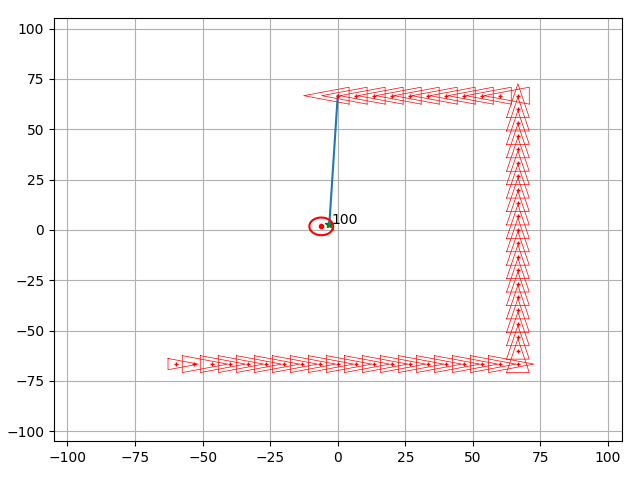
\includegraphics{fig6-1-2.png}
\end{figure}

Fig. 1: Example run of the EKF algorithmn for mapping (only one
landmark). it shows the true pose (in red), the real pose of the
landmark (as a green star), and the estimation from the EKF algorithm
(pose and confidence ellipse).

    \begin{tcolorbox}[breakable, size=fbox, boxrule=1pt, pad at break*=1mm,colback=cellbackground, colframe=cellborder]
\prompt{In}{incolor}{14}{\boxspacing}
\begin{Verbatim}[commandchars=\\\{\}]
\PY{k}{def} \PY{n+nf}{demo\PYZus{}ekf\PYZus{}mapping}\PY{p}{(}\PY{n}{robot}\PY{p}{,}
                     \PY{n}{Map}\PY{p}{,}
                     \PY{n}{nLandmarks}\PY{p}{,}
                     \PY{n}{mode}\PY{o}{=}\PY{l+s+s1}{\PYZsq{}}\PY{l+s+s1}{non\PYZus{}stop}\PY{l+s+s1}{\PYZsq{}}\PY{p}{,}
                     \PY{n}{logger}\PY{o}{=}\PY{k+kc}{None}\PY{p}{,}
                     \PY{n}{nSteps}\PY{o}{=}\PY{l+m+mi}{100}\PY{p}{,} \PY{c+c1}{\PYZsh{} Number of motions}
                     \PY{n}{turning}\PY{o}{=} \PY{l+m+mi}{40}\PY{p}{,} \PY{c+c1}{\PYZsh{} Number of motions before turning (square path)}
                     \PY{n}{print\PYZus{}each}\PY{o}{=}\PY{l+m+mi}{2}\PY{p}{)}\PY{p}{:}
    
    \PY{o}{\PYZpc{}}\PY{k}{matplotlib} notebook
    \PY{k}{if} \PY{n}{mode} \PY{o}{==} \PY{l+s+s1}{\PYZsq{}}\PY{l+s+s1}{step\PYZus{}by\PYZus{}step}\PY{l+s+s1}{\PYZsq{}}\PY{p}{:}
        \PY{n}{matplotlib}\PY{o}{.}\PY{n}{use}\PY{p}{(}\PY{l+s+s1}{\PYZsq{}}\PY{l+s+s1}{TkAgg}\PY{l+s+s1}{\PYZsq{}}\PY{p}{)}

    \PY{c+c1}{\PYZsh{} storing the number of times a landmark has been seen}
    \PY{c+c1}{\PYZsh{} also store the handler to the graphical info shown}
    \PY{n}{canvas} \PY{o}{=} \PY{n}{MapCanvas}\PY{p}{(}\PY{n}{nLandmarks}\PY{p}{)}
    
    \PY{n}{canvas}\PY{o}{.}\PY{n}{ax}\PY{o}{.}\PY{n}{plot}\PY{p}{(}\PY{n}{Map}\PY{p}{[}\PY{l+m+mi}{0}\PY{p}{,} \PY{p}{:}\PY{p}{]}\PY{p}{,} \PY{n}{Map}\PY{p}{[}\PY{l+m+mi}{1}\PY{p}{,} \PY{p}{:}\PY{p}{]}\PY{p}{,} \PY{l+s+s1}{\PYZsq{}}\PY{l+s+s1}{g*}\PY{l+s+s1}{\PYZsq{}}\PY{p}{)}
    \PY{n}{hObsLine} \PY{o}{=} \PY{n}{canvas}\PY{o}{.}\PY{n}{ax}\PY{o}{.}\PY{n}{plot}\PY{p}{(}\PY{p}{[}\PY{l+m+mi}{0}\PY{p}{,}\PY{l+m+mi}{0}\PY{p}{]}\PY{p}{,} \PY{p}{[}\PY{l+m+mi}{0}\PY{p}{,}\PY{l+m+mi}{0}\PY{p}{]}\PY{p}{,} \PY{n}{linestyle}\PY{o}{=}\PY{l+s+s1}{\PYZsq{}}\PY{l+s+s1}{:}\PY{l+s+s1}{\PYZsq{}}\PY{p}{)}
    
    \PY{c+c1}{\PYZsh{} Control action}
    \PY{n}{u} \PY{o}{=} \PY{n}{np}\PY{o}{.}\PY{n}{zeros}\PY{p}{(}\PY{p}{(}\PY{l+m+mi}{3}\PY{p}{,} \PY{l+m+mi}{1}\PY{p}{)}\PY{p}{)}
    \PY{n}{u}\PY{p}{[}\PY{l+m+mi}{0}\PY{p}{]} \PY{o}{=} \PY{p}{(}\PY{l+m+mf}{2.}\PY{o}{*}\PY{n}{MapSize}\PY{o}{/}\PY{l+m+mf}{1.5}\PY{p}{)}\PY{o}{/}\PY{n}{turning}
    \PY{n}{u}\PY{p}{[}\PY{l+m+mi}{1}\PY{p}{]} \PY{o}{=} \PY{l+m+mf}{0.}
    
    \PY{c+c1}{\PYZsh{} Start the loop!}
    \PY{k}{for} \PY{n}{k} \PY{o+ow}{in} \PY{n+nb}{range}\PY{p}{(}\PY{n}{nSteps}\PY{p}{)}\PY{p}{:}
        \PY{c+c1}{\PYZsh{}}
        \PY{c+c1}{\PYZsh{} Move the robot}
        \PY{c+c1}{\PYZsh{}}
        \PY{n}{u}\PY{p}{[}\PY{l+m+mi}{2}\PY{p}{]}\PY{o}{=}\PY{l+m+mf}{0.}
        \PY{k}{if} \PY{n}{k}\PY{o}{\PYZpc{}}\PY{k}{turning} == turning\PYZhy{}1:
            \PY{n}{u}\PY{p}{[}\PY{l+m+mi}{2}\PY{p}{]} \PY{o}{=} \PY{n}{np}\PY{o}{.}\PY{n}{pi}\PY{o}{/}\PY{l+m+mi}{2}
        
        \PY{n}{robot}\PY{o}{.}\PY{n}{step}\PY{p}{(}\PY{n}{u}\PY{p}{)} \PY{c+c1}{\PYZsh{} Perfectly known robot pose}
        
        \PY{n}{z}\PY{p}{,} \PY{n}{iLandmark} \PY{o}{=} \PY{n}{robot}\PY{o}{.}\PY{n}{get\PYZus{}random\PYZus{}observation}\PY{p}{(}\PY{n}{world}\PY{o}{=}\PY{n}{Map}\PY{p}{)}
        
        \PY{c+c1}{\PYZsh{} Update the \PYZdq{}observedtimes\PYZdq{} for the feature and plot the reading}
        \PY{n}{canvas}\PY{o}{.}\PY{n}{increment\PYZus{}observed\PYZus{}times}\PY{p}{(}\PY{n}{iLandmark}\PY{p}{)}
        \PY{n}{canvas}\PY{o}{.}\PY{n}{PlotNumberOfReadings}\PY{p}{(}\PY{n}{robot}\PY{o}{.}\PY{n}{true\PYZus{}pose}\PY{p}{,} \PY{n}{iLandmark}\PY{p}{,} \PY{n}{Map}\PY{p}{)}
        
        \PY{n}{EKFMapping}\PY{p}{(}\PY{n}{robot}\PY{p}{,} \PY{n}{z}\PY{p}{,} \PY{n}{iLandmark}\PY{p}{)}
        
        \PY{c+c1}{\PYZsh{} Print map evolution each 5 steps}
        \PY{k}{if} \PY{o+ow}{not} \PY{n}{k}\PY{o}{\PYZpc{}}\PY{k}{5}:
            \PY{k}{with} \PY{n}{np}\PY{o}{.}\PY{n}{printoptions}\PY{p}{(}\PY{n}{precision}\PY{o}{=}\PY{l+m+mi}{3}\PY{p}{)}\PY{p}{:}
                \PY{n+nb}{print}\PY{p}{(}\PY{l+s+s1}{\PYZsq{}}\PY{l+s+s1}{Iteration: }\PY{l+s+s1}{\PYZsq{}} \PY{o}{+} \PY{n+nb}{str}\PY{p}{(}\PY{n}{k}\PY{p}{)}\PY{p}{)}
                \PY{n+nb}{print}\PY{p}{(}\PY{l+s+s1}{\PYZsq{}}\PY{l+s+s1}{Estimated xEst:}\PY{l+s+se}{\PYZbs{}n}\PY{l+s+s1}{\PYZsq{}} \PY{o}{+} \PY{n+nb}{str}\PY{p}{(}\PY{n}{robot}\PY{o}{.}\PY{n}{xEst}\PY{p}{)}\PY{p}{)}
                \PY{n+nb}{print}\PY{p}{(}\PY{l+s+s1}{\PYZsq{}}\PY{l+s+s1}{Estimated PEst:}\PY{l+s+se}{\PYZbs{}n}\PY{l+s+s1}{\PYZsq{}} \PY{o}{+} \PY{n+nb}{str}\PY{p}{(}\PY{n}{robot}\PY{o}{.}\PY{n}{PEst}\PY{p}{)}\PY{p}{)}
                \PY{n+nb}{print}\PY{p}{(}\PY{l+s+s1}{\PYZsq{}}\PY{l+s+s1}{\PYZhy{}\PYZhy{}\PYZhy{}\PYZhy{}\PYZhy{}\PYZhy{}\PYZhy{}\PYZhy{}\PYZhy{}\PYZhy{}\PYZhy{}\PYZhy{}\PYZhy{}\PYZhy{}\PYZhy{}\PYZhy{}\PYZhy{}\PYZhy{}\PYZhy{}\PYZhy{}\PYZhy{}\PYZhy{}\PYZhy{}\PYZhy{}\PYZhy{}\PYZhy{}\PYZhy{}\PYZhy{}\PYZhy{}\PYZhy{}\PYZhy{}\PYZhy{}\PYZhy{}}\PY{l+s+s1}{\PYZsq{}}\PY{p}{)}
        
        \PY{c+c1}{\PYZsh{} Log important values}
        \PY{k}{if} \PY{n}{logger} \PY{o+ow}{is} \PY{o+ow}{not} \PY{k+kc}{None}\PY{p}{:}
            \PY{n}{logger}\PY{o}{.}\PY{n}{log}\PY{p}{(}\PY{n}{k}\PY{p}{,} \PY{n}{robot}\PY{p}{,} \PY{n}{Map}\PY{p}{)}
        
        \PY{c+c1}{\PYZsh{} Drawings}
        \PY{k}{if} \PY{n}{k}\PY{o}{\PYZpc{}}\PY{k}{print\PYZus{}each} == print\PYZus{}each\PYZhy{}1:
            \PY{n}{DrawRobot}\PY{p}{(}\PY{n}{canvas}\PY{o}{.}\PY{n}{fig}\PY{p}{,} \PY{n}{canvas}\PY{o}{.}\PY{n}{ax}\PY{p}{,}\PY{n}{robot}\PY{o}{.}\PY{n}{true\PYZus{}pose}\PY{p}{,} \PY{l+s+s1}{\PYZsq{}}\PY{l+s+s1}{r}\PY{l+s+s1}{\PYZsq{}}\PY{p}{)}\PY{c+c1}{\PYZsh{}plot(xVehicleTrue(1),xVehicleTrue(2),\PYZsq{}r*\PYZsq{})}
            \PY{n}{canvas}\PY{o}{.}\PY{n}{DoMapGraphics}\PY{p}{(}\PY{n}{robot}\PY{p}{)} \PY{c+c1}{\PYZsh{} Draw estimated poitns (in black) and ellipses}
            \PY{n}{plt}\PY{o}{.}\PY{n}{axis}\PY{p}{(}\PY{p}{[}\PY{o}{\PYZhy{}}\PY{n}{MapSize}\PY{o}{\PYZhy{}}\PY{l+m+mi}{5}\PY{p}{,} \PY{n}{MapSize}\PY{o}{+}\PY{l+m+mi}{5}\PY{p}{,} \PY{o}{\PYZhy{}}\PY{n}{MapSize}\PY{o}{\PYZhy{}}\PY{l+m+mi}{5}\PY{p}{,} \PY{n}{MapSize}\PY{o}{+}\PY{l+m+mi}{5}\PY{p}{]}\PY{p}{)} \PY{c+c1}{\PYZsh{} Set limits again}
            \PY{n}{plt}\PY{o}{.}\PY{n}{draw}\PY{p}{(}\PY{p}{)}
            
            \PY{k}{if} \PY{n}{mode} \PY{o}{==} \PY{l+s+s1}{\PYZsq{}}\PY{l+s+s1}{step\PYZus{}by\PYZus{}step}\PY{l+s+s1}{\PYZsq{}}\PY{p}{:}
                \PY{n}{plt}\PY{o}{.}\PY{n}{waitforbuttonpress}\PY{p}{(}\PY{o}{\PYZhy{}}\PY{l+m+mi}{1}\PY{p}{)}
            \PY{k}{elif} \PY{n}{mode} \PY{o}{==} \PY{l+s+s1}{\PYZsq{}}\PY{l+s+s1}{visualize\PYZus{}process}\PY{l+s+s1}{\PYZsq{}}\PY{p}{:}
                \PY{n}{plt}\PY{o}{.}\PY{n}{pause}\PY{p}{(}\PY{l+m+mf}{0.2}\PY{p}{)}
            \PY{k}{elif} \PY{n}{mode} \PY{o}{==} \PY{l+s+s1}{\PYZsq{}}\PY{l+s+s1}{non\PYZus{}stop}\PY{l+s+s1}{\PYZsq{}}\PY{p}{:}
                \PY{k}{pass} \PY{c+c1}{\PYZsh{} non stop!}

    \PY{c+c1}{\PYZsh{} Final drawings}
    \PY{o}{\PYZpc{}}\PY{k}{matplotlib} inline
    \PY{k}{if} \PY{n}{logger} \PY{o+ow}{is} \PY{o+ow}{not} \PY{k+kc}{None}\PY{p}{:}
        \PY{n}{logger}\PY{o}{.}\PY{n}{plot}\PY{p}{(}\PY{p}{)}
\end{Verbatim}
\end{tcolorbox}

    \begin{tcolorbox}[breakable, size=fbox, boxrule=1pt, pad at break*=1mm,colback=cellbackground, colframe=cellborder]
\prompt{In}{incolor}{15}{\boxspacing}
\begin{Verbatim}[commandchars=\\\{\}]
\PY{c+c1}{\PYZsh{}mode = \PYZsq{}step\PYZus{}by\PYZus{}step\PYZsq{}}
\PY{n}{mode} \PY{o}{=} \PY{l+s+s1}{\PYZsq{}}\PY{l+s+s1}{visualize\PYZus{}process}\PY{l+s+s1}{\PYZsq{}}
\PY{c+c1}{\PYZsh{}mode = \PYZsq{}non\PYZus{}stop\PYZsq{}}

\PY{c+c1}{\PYZsh{} WORLD MAP}
\PY{c+c1}{\PYZsh{} Num features/landmarks considered within the map}
\PY{n}{nLandmarks} \PY{o}{=} \PY{l+m+mi}{1}
\PY{c+c1}{\PYZsh{} Generation of the map}
\PY{n}{MapSize} \PY{o}{=} \PY{l+m+mi}{100}
\PY{n}{Map} \PY{o}{=} \PY{n}{MapSize}\PY{o}{*}\PY{n}{random}\PY{o}{.}\PY{n}{rand}\PY{p}{(}\PY{l+m+mi}{2}\PY{p}{,}\PY{n}{nLandmarks}\PY{p}{)}\PY{o}{\PYZhy{}}\PY{n}{MapSize}\PY{o}{/}\PY{l+m+mi}{2}

\PY{c+c1}{\PYZsh{} ROBOT}
\PY{c+c1}{\PYZsh{} Covariances for our very bad\PYZam{}expensive sensor (in the system \PYZlt{}d,theta\PYZgt{})}
\PY{n}{Sigma\PYZus{}r} \PY{o}{=} \PY{l+m+mf}{8.0}
\PY{n}{Sigma\PYZus{}theta} \PY{o}{=} \PY{l+m+mi}{8}\PY{o}{*}\PY{n}{np}\PY{o}{.}\PY{n}{pi}\PY{o}{/}\PY{l+m+mi}{180}
\PY{c+c1}{\PYZsh{} Initial robot pose}
\PY{n}{xVehicleTrue} \PY{o}{=} \PY{n}{np}\PY{o}{.}\PY{n}{vstack}\PY{p}{(}\PY{p}{[}\PY{o}{\PYZhy{}}\PY{n}{MapSize}\PY{o}{/}\PY{l+m+mf}{1.5}\PY{p}{,} \PY{o}{\PYZhy{}}\PY{n}{MapSize}\PY{o}{/}\PY{l+m+mf}{1.5}\PY{p}{,} \PY{l+m+mf}{0.}\PY{p}{]}\PY{p}{)} \PY{c+c1}{\PYZsh{} We know the exact robot pose at any moment}

\PY{n}{robot} \PY{o}{=} \PY{n}{EFKMappingRobot}\PY{p}{(}\PY{n}{xVehicleTrue}\PY{p}{,} \PY{n}{Sigma\PYZus{}r}\PY{p}{,} \PY{n}{Sigma\PYZus{}theta}\PY{p}{,} \PY{n}{nLandmarks}\PY{p}{)}

\PY{n}{demo\PYZus{}ekf\PYZus{}mapping}\PY{p}{(}\PY{n}{robot}\PY{p}{,} \PY{n}{Map} \PY{p}{,}\PY{n}{nLandmarks}\PY{p}{,} \PY{n}{mode}\PY{o}{=}\PY{n}{mode}\PY{p}{)}
\end{Verbatim}
\end{tcolorbox}

    
\begin{figure}
\centering
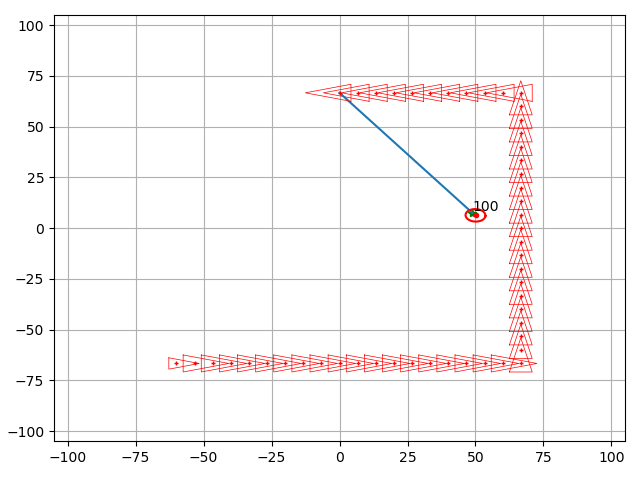
\includegraphics{3.png}
\end{figure}
    
    \begin{Verbatim}[commandchars=\\\{\}]
Iteration: 0
Estimated xEst:
[[48.245]
 [ 3.712]]
Estimated PEst:
[[ 142.349 -124.215]
 [-124.215  260.929]]
---------------------------------
Iteration: 5
Estimated xEst:
[[54.879]
 [ 2.38 ]]
Estimated PEst:
[[ 22.595 -18.926]
 [-18.926  40.709]]
---------------------------------
Iteration: 10
Estimated xEst:
[[52.347]
 [ 5.644]]
Estimated PEst:
[[12.578 -9.412]
 [-9.412 18.999]]
---------------------------------
Iteration: 15
Estimated xEst:
[[51.694]
 [ 9.218]]
Estimated PEst:
[[ 8.514 -5.629]
 [-5.629 11.107]]
---------------------------------
Iteration: 20
Estimated xEst:
[[51.927]
 [ 8.834]]
Estimated PEst:
[[ 6.309 -3.624]
 [-3.624  7.174]]
---------------------------------
Iteration: 25
Estimated xEst:
[[51.575]
 [ 9.319]]
Estimated PEst:
[[ 4.909 -2.405]
 [-2.405  4.945]]
---------------------------------
Iteration: 30
Estimated xEst:
[[50.808]
 [ 8.553]]
Estimated PEst:
[[ 3.924 -1.607]
 [-1.607  3.592]]
---------------------------------
Iteration: 35
Estimated xEst:
[[50.636]
 [ 8.147]]
Estimated PEst:
[[ 3.218 -1.087]
 [-1.087  2.756]]
---------------------------------
Iteration: 40
Estimated xEst:
[[51.061]
 [ 7.107]]
Estimated PEst:
[[ 2.717 -0.748]
 [-0.748  2.222]]
---------------------------------
Iteration: 45
Estimated xEst:
[[50.842]
 [ 7.412]]
Estimated PEst:
[[ 2.266 -0.529]
 [-0.529  1.867]]
---------------------------------
Iteration: 50
Estimated xEst:
[[50.337]
 [ 7.85 ]]
Estimated PEst:
[[ 1.81  -0.406]
 [-0.406  1.613]]
---------------------------------
Iteration: 55
Estimated xEst:
[[50.198]
 [ 6.784]]
Estimated PEst:
[[ 1.378 -0.402]
 [-0.402  1.383]]
---------------------------------
Iteration: 60
Estimated xEst:
[[50.394]
 [ 5.648]]
Estimated PEst:
[[ 1.166 -0.387]
 [-0.387  0.873]]
---------------------------------
Iteration: 65
Estimated xEst:
[[49.906]
 [ 6.551]]
Estimated PEst:
[[ 0.862 -0.102]
 [-0.102  0.507]]
---------------------------------
Iteration: 70
Estimated xEst:
[[50.53 ]
 [ 6.328]]
Estimated PEst:
[[ 0.708 -0.04 ]
 [-0.04   0.459]]
---------------------------------
Iteration: 75
Estimated xEst:
[[50.575]
 [ 6.317]]
Estimated PEst:
[[ 0.647 -0.029]
 [-0.029  0.44 ]]
---------------------------------
Iteration: 80
Estimated xEst:
[[50.477]
 [ 6.181]]
Estimated PEst:
[[ 0.617 -0.026]
 [-0.026  0.425]]
---------------------------------
Iteration: 85
Estimated xEst:
[[50.574]
 [ 6.128]]
Estimated PEst:
[[ 0.591 -0.025]
 [-0.025  0.412]]
---------------------------------
Iteration: 90
Estimated xEst:
[[50.147]
 [ 6.16 ]]
Estimated PEst:
[[ 0.569 -0.022]
 [-0.022  0.399]]
---------------------------------
Iteration: 95
Estimated xEst:
[[50.142]
 [ 6.167]]
Estimated PEst:
[[ 0.549 -0.019]
 [-0.019  0.387]]
---------------------------------
    \end{Verbatim}

    \hypertarget{considering-a-larger-number-of-landmarks}{%
\subsubsection{Considering a larger number of
landmarks}\label{considering-a-larger-number-of-landmarks}}

Once our EKF implementation is working with one landmark, let's try it
in a scenario with 5 landmarks. Again, the content of the \texttt{xEst}
and \texttt{Pest} is shown after each 5 iterations of the algorithm.

\begin{figure}
\centering
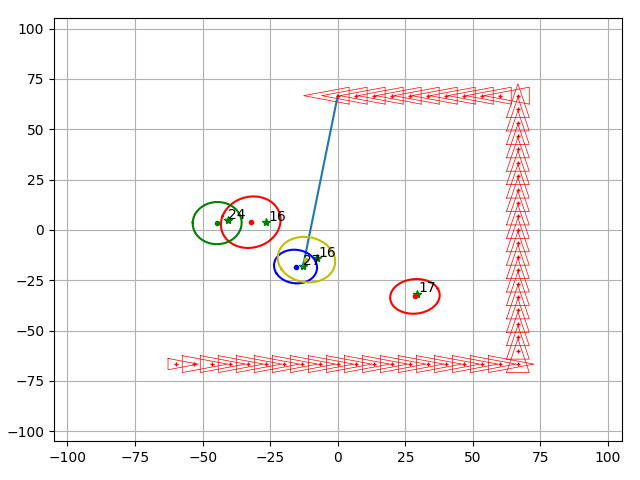
\includegraphics{fig6-1-3.png}
\end{figure}

Fig. 2: Execution of the EKF algorithmn for mapping (multiple
landmarks). Same as in Fig 1., each landmark is accompanied by a number
of times observed.

    \begin{tcolorbox}[breakable, size=fbox, boxrule=1pt, pad at break*=1mm,colback=cellbackground, colframe=cellborder]
\prompt{In}{incolor}{17}{\boxspacing}
\begin{Verbatim}[commandchars=\\\{\}]
\PY{c+c1}{\PYZsh{}mode = \PYZsq{}step\PYZus{}by\PYZus{}step\PYZsq{}}
\PY{n}{mode} \PY{o}{=} \PY{l+s+s1}{\PYZsq{}}\PY{l+s+s1}{visualize\PYZus{}process}\PY{l+s+s1}{\PYZsq{}}
\PY{c+c1}{\PYZsh{}mode = \PYZsq{}non\PYZus{}stop\PYZsq{}}

\PY{c+c1}{\PYZsh{} WORLD MAP}
\PY{c+c1}{\PYZsh{} Num features/landmarks considered within the map}
\PY{n}{nLandmarks} \PY{o}{=} \PY{l+m+mi}{5}
\PY{c+c1}{\PYZsh{} Generation of the map}
\PY{n}{MapSize} \PY{o}{=} \PY{l+m+mi}{100}
\PY{n}{Map} \PY{o}{=} \PY{n}{MapSize}\PY{o}{*}\PY{n}{random}\PY{o}{.}\PY{n}{rand}\PY{p}{(}\PY{l+m+mi}{2}\PY{p}{,}\PY{n}{nLandmarks}\PY{p}{)}\PY{o}{\PYZhy{}}\PY{n}{MapSize}\PY{o}{/}\PY{l+m+mi}{2}

\PY{c+c1}{\PYZsh{} ROBOT}
\PY{c+c1}{\PYZsh{} Covariances for our very bad\PYZam{}expensive sensor (in the system \PYZlt{}d,theta\PYZgt{})}
\PY{n}{Sigma\PYZus{}r} \PY{o}{=} \PY{l+m+mf}{8.0}
\PY{n}{Sigma\PYZus{}theta} \PY{o}{=} \PY{l+m+mi}{7}\PY{o}{*}\PY{n}{np}\PY{o}{.}\PY{n}{pi}\PY{o}{/}\PY{l+m+mi}{180}
\PY{c+c1}{\PYZsh{} Initial robot pose}
\PY{n}{xVehicleTrue} \PY{o}{=} \PY{n}{np}\PY{o}{.}\PY{n}{vstack}\PY{p}{(}\PY{p}{[}\PY{o}{\PYZhy{}}\PY{n}{MapSize}\PY{o}{/}\PY{l+m+mf}{1.5}\PY{p}{,} \PY{o}{\PYZhy{}}\PY{n}{MapSize}\PY{o}{/}\PY{l+m+mf}{1.5}\PY{p}{,} \PY{l+m+mf}{0.}\PY{p}{]}\PY{p}{)} \PY{c+c1}{\PYZsh{} We know the exact robot pose at any moment}

\PY{n}{robot} \PY{o}{=} \PY{n}{EFKMappingRobot}\PY{p}{(}\PY{n}{xVehicleTrue}\PY{p}{,} \PY{n}{Sigma\PYZus{}r}\PY{p}{,} \PY{n}{Sigma\PYZus{}theta}\PY{p}{,} \PY{n}{nLandmarks}\PY{p}{)}

\PY{n}{demo\PYZus{}ekf\PYZus{}mapping}\PY{p}{(}\PY{n}{robot}\PY{p}{,} \PY{n}{Map} \PY{p}{,}\PY{n}{nLandmarks}\PY{p}{,} \PY{n}{mode}\PY{o}{=}\PY{n}{mode}\PY{p}{)}
\end{Verbatim}
\end{tcolorbox}

    
\begin{figure}
\centering
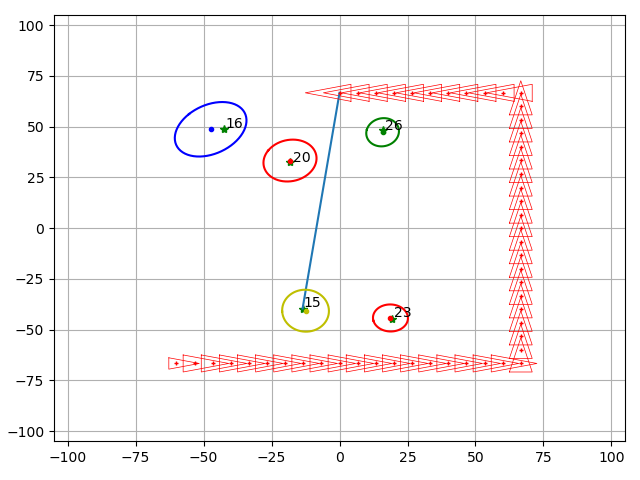
\includegraphics{4.png}
\end{figure}

    
    \begin{Verbatim}[commandchars=\\\{\}]
Iteration: 0
Estimated xEst:
[[ 23.676]
 [-50.071]]
Estimated PEst:
[[ 65.864  -9.774]
 [ -9.774 115.247]]
---------------------------------
Iteration: 5
Estimated xEst:
[[ 23.676]
 [-50.071]
 [-65.682]
 [ 47.731]
 [-10.107]
 [-42.036]
 [ 38.702]
 [ 31.415]
 [ -3.238]
 [ 22.936]]
Estimated PEst:
[[  65.864   -9.774    0.       0.       0.       0.       0.       0.
     0.       0.   ]
 [  -9.774  115.247    0.       0.       0.       0.       0.       0.
     0.       0.   ]
 [   0.       0.     195.496    6.532    0.       0.       0.       0.
     0.       0.   ]
 [   0.       0.       6.532   64.324    0.       0.       0.       0.
     0.       0.   ]
 [   0.       0.       0.       0.      28.039    7.267    0.       0.
     0.       0.   ]
 [   0.       0.       0.       0.       7.267   18.275    0.       0.
     0.       0.   ]
 [   0.       0.       0.       0.       0.       0.     173.556 -102.804
     0.       0.   ]
 [   0.       0.       0.       0.       0.       0.    -102.804  160.467
     0.       0.   ]
 [   0.       0.       0.       0.       0.       0.       0.       0.
   133.538  -36.29 ]
 [   0.       0.       0.       0.       0.       0.       0.       0.
   -36.29    82.939]]
---------------------------------
Iteration: 10
Estimated xEst:
[[ 23.676]
 [-50.071]
 [-62.357]
 [ 49.037]
 [-10.107]
 [-42.036]
 [ 21.718]
 [ 50.756]
 [ -3.238]
 [ 22.936]]
Estimated PEst:
[[ 65.864  -9.774   0.      0.      0.      0.      0.      0.      0.
    0.   ]
 [ -9.774 115.247   0.      0.      0.      0.      0.      0.      0.
    0.   ]
 [  0.      0.     97.434   8.944   0.      0.      0.      0.      0.
    0.   ]
 [  0.      0.      8.944  33.386   0.      0.      0.      0.      0.
    0.   ]
 [  0.      0.      0.      0.     28.039   7.267   0.      0.      0.
    0.   ]
 [  0.      0.      0.      0.      7.267  18.275   0.      0.      0.
    0.   ]
 [  0.      0.      0.      0.      0.      0.     37.086 -15.549   0.
    0.   ]
 [  0.      0.      0.      0.      0.      0.    -15.549  23.005   0.
    0.   ]
 [  0.      0.      0.      0.      0.      0.      0.      0.    133.538
  -36.29 ]
 [  0.      0.      0.      0.      0.      0.      0.      0.    -36.29
   82.939]]
---------------------------------
Iteration: 15
Estimated xEst:
[[ 19.153]
 [-47.067]
 [-62.357]
 [ 49.037]
 [-11.288]
 [-39.241]
 [ 21.252]
 [ 52.619]
 [ -2.342]
 [ 32.878]]
Estimated PEst:
[[ 29.615   5.272   0.      0.      0.      0.      0.      0.      0.
    0.   ]
 [  5.272  23.009   0.      0.      0.      0.      0.      0.      0.
    0.   ]
 [  0.      0.     97.434   8.944   0.      0.      0.      0.      0.
    0.   ]
 [  0.      0.      8.944  33.386   0.      0.      0.      0.      0.
    0.   ]
 [  0.      0.      0.      0.      8.336   3.799   0.      0.      0.
    0.   ]
 [  0.      0.      0.      0.      3.799  13.864   0.      0.      0.
    0.   ]
 [  0.      0.      0.      0.      0.      0.     27.299 -10.249   0.
    0.   ]
 [  0.      0.      0.      0.      0.      0.    -10.249  15.115   0.
    0.   ]
 [  0.      0.      0.      0.      0.      0.      0.      0.     62.786
  -10.99 ]
 [  0.      0.      0.      0.      0.      0.      0.      0.    -10.99
   36.343]]
---------------------------------
Iteration: 20
Estimated xEst:
[[ 19.21 ]
 [-47.37 ]
 [-59.693]
 [ 43.746]
 [-13.491]
 [-41.81 ]
 [ 21.533]
 [ 50.524]
 [ -2.342]
 [ 32.878]]
Estimated PEst:
[[ 10.233   5.225   0.      0.      0.      0.      0.      0.      0.
    0.   ]
 [  5.225   9.757   0.      0.      0.      0.      0.      0.      0.
    0.   ]
 [  0.      0.     64.346  10.692   0.      0.      0.      0.      0.
    0.   ]
 [  0.      0.     10.692  24.422   0.      0.      0.      0.      0.
    0.   ]
 [  0.      0.      0.      0.      4.95    0.754   0.      0.      0.
    0.   ]
 [  0.      0.      0.      0.      0.754   9.476   0.      0.      0.
    0.   ]
 [  0.      0.      0.      0.      0.      0.     23.825  -8.142   0.
    0.   ]
 [  0.      0.      0.      0.      0.      0.     -8.142  12.405   0.
    0.   ]
 [  0.      0.      0.      0.      0.      0.      0.      0.     62.786
  -10.99 ]
 [  0.      0.      0.      0.      0.      0.      0.      0.    -10.99
   36.343]]
---------------------------------
Iteration: 25
Estimated xEst:
[[ 16.959]
 [-47.73 ]
 [-59.7  ]
 [ 48.97 ]
 [-13.491]
 [-41.81 ]
 [ 19.636]
 [ 50.606]
 [ -7.71 ]
 [ 33.154]]
Estimated PEst:
[[ 3.93   2.29   0.     0.     0.     0.     0.     0.     0.     0.   ]
 [ 2.29   7.607  0.     0.     0.     0.     0.     0.     0.     0.   ]
 [ 0.     0.    37.702 10.021  0.     0.     0.     0.     0.     0.   ]
 [ 0.     0.    10.021 17.298  0.     0.     0.     0.     0.     0.   ]
 [ 0.     0.     0.     0.     4.95   0.754  0.     0.     0.     0.   ]
 [ 0.     0.     0.     0.     0.754  9.476  0.     0.     0.     0.   ]
 [ 0.     0.     0.     0.     0.     0.    20.829 -6.321  0.     0.   ]
 [ 0.     0.     0.     0.     0.     0.    -6.321 10.287  0.     0.   ]
 [ 0.     0.     0.     0.     0.     0.     0.     0.    43.003 -3.853]
 [ 0.     0.     0.     0.     0.     0.     0.     0.    -3.853 22.796]]
---------------------------------
Iteration: 30
Estimated xEst:
[[ 17.37 ]
 [-45.866]
 [-53.126]
 [ 50.505]
 [-13.491]
 [-41.81 ]
 [ 18.776]
 [ 48.798]
 [ -7.71 ]
 [ 33.154]]
Estimated PEst:
[[ 2.897  0.758  0.     0.     0.     0.     0.     0.     0.     0.   ]
 [ 0.758  4.881  0.     0.     0.     0.     0.     0.     0.     0.   ]
 [ 0.     0.    27.279  9.036  0.     0.     0.     0.     0.     0.   ]
 [ 0.     0.     9.036 14.015  0.     0.     0.     0.     0.     0.   ]
 [ 0.     0.     0.     0.     4.95   0.754  0.     0.     0.     0.   ]
 [ 0.     0.     0.     0.     0.754  9.476  0.     0.     0.     0.   ]
 [ 0.     0.     0.     0.     0.     0.    16.362 -3.732  0.     0.   ]
 [ 0.     0.     0.     0.     0.     0.    -3.732  7.493  0.     0.   ]
 [ 0.     0.     0.     0.     0.     0.     0.     0.    43.003 -3.853]
 [ 0.     0.     0.     0.     0.     0.     0.     0.    -3.853 22.796]]
---------------------------------
Iteration: 35
Estimated xEst:
[[ 17.571]
 [-44.047]
 [-52.08 ]
 [ 47.905]
 [-13.491]
 [-41.81 ]
 [ 18.776]
 [ 48.798]
 [ -7.71 ]
 [ 33.154]]
Estimated PEst:
[[ 2.200e+00 -1.002e-02  0.000e+00  0.000e+00  0.000e+00  0.000e+00
   0.000e+00  0.000e+00  0.000e+00  0.000e+00]
 [-1.002e-02  3.031e+00  0.000e+00  0.000e+00  0.000e+00  0.000e+00
   0.000e+00  0.000e+00  0.000e+00  0.000e+00]
 [ 0.000e+00  0.000e+00  2.136e+01  8.213e+00  0.000e+00  0.000e+00
   0.000e+00  0.000e+00  0.000e+00  0.000e+00]
 [ 0.000e+00  0.000e+00  8.213e+00  1.217e+01  0.000e+00  0.000e+00
   0.000e+00  0.000e+00  0.000e+00  0.000e+00]
 [ 0.000e+00  0.000e+00  0.000e+00  0.000e+00  4.950e+00  7.535e-01
   0.000e+00  0.000e+00  0.000e+00  0.000e+00]
 [ 0.000e+00  0.000e+00  0.000e+00  0.000e+00  7.535e-01  9.476e+00
   0.000e+00  0.000e+00  0.000e+00  0.000e+00]
 [ 0.000e+00  0.000e+00  0.000e+00  0.000e+00  0.000e+00  0.000e+00
   1.636e+01 -3.732e+00  0.000e+00  0.000e+00]
 [ 0.000e+00  0.000e+00  0.000e+00  0.000e+00  0.000e+00  0.000e+00
  -3.732e+00  7.493e+00  0.000e+00  0.000e+00]
 [ 0.000e+00  0.000e+00  0.000e+00  0.000e+00  0.000e+00  0.000e+00
   0.000e+00  0.000e+00  4.300e+01 -3.853e+00]
 [ 0.000e+00  0.000e+00  0.000e+00  0.000e+00  0.000e+00  0.000e+00
   0.000e+00  0.000e+00 -3.853e+00  2.280e+01]]
---------------------------------
Iteration: 40
Estimated xEst:
[[ 17.571]
 [-44.047]
 [-52.08 ]
 [ 47.905]
 [-14.039]
 [-41.721]
 [ 18.051]
 [ 48.418]
 [-10.091]
 [ 36.081]]
Estimated PEst:
[[ 2.200e+00 -1.002e-02  0.000e+00  0.000e+00  0.000e+00  0.000e+00
   0.000e+00  0.000e+00  0.000e+00  0.000e+00]
 [-1.002e-02  3.031e+00  0.000e+00  0.000e+00  0.000e+00  0.000e+00
   0.000e+00  0.000e+00  0.000e+00  0.000e+00]
 [ 0.000e+00  0.000e+00  2.136e+01  8.213e+00  0.000e+00  0.000e+00
   0.000e+00  0.000e+00  0.000e+00  0.000e+00]
 [ 0.000e+00  0.000e+00  8.213e+00  1.217e+01  0.000e+00  0.000e+00
   0.000e+00  0.000e+00  0.000e+00  0.000e+00]
 [ 0.000e+00  0.000e+00  0.000e+00  0.000e+00  4.604e+00  6.704e-01
   0.000e+00  0.000e+00  0.000e+00  0.000e+00]
 [ 0.000e+00  0.000e+00  0.000e+00  0.000e+00  6.704e-01  8.479e+00
   0.000e+00  0.000e+00  0.000e+00  0.000e+00]
 [ 0.000e+00  0.000e+00  0.000e+00  0.000e+00  0.000e+00  0.000e+00
   1.188e+01 -1.398e+00  0.000e+00  0.000e+00]
 [ 0.000e+00  0.000e+00  0.000e+00  0.000e+00  0.000e+00  0.000e+00
  -1.398e+00  5.354e+00  0.000e+00  0.000e+00]
 [ 0.000e+00  0.000e+00  0.000e+00  0.000e+00  0.000e+00  0.000e+00
   0.000e+00  0.000e+00  3.145e+01  7.148e-01]
 [ 0.000e+00  0.000e+00  0.000e+00  0.000e+00  0.000e+00  0.000e+00
   0.000e+00  0.000e+00  7.148e-01  1.774e+01]]
---------------------------------
Iteration: 45
Estimated xEst:
[[ 17.571]
 [-44.047]
 [-47.734]
 [ 48.61 ]
 [-13.299]
 [-42.38 ]
 [ 17.175]
 [ 48.235]
 [-11.958]
 [ 36.508]]
Estimated PEst:
[[ 2.200e+00 -1.002e-02  0.000e+00  0.000e+00  0.000e+00  0.000e+00
   0.000e+00  0.000e+00  0.000e+00  0.000e+00]
 [-1.002e-02  3.031e+00  0.000e+00  0.000e+00  0.000e+00  0.000e+00
   0.000e+00  0.000e+00  0.000e+00  0.000e+00]
 [ 0.000e+00  0.000e+00  1.695e+01  7.365e+00  0.000e+00  0.000e+00
   0.000e+00  0.000e+00  0.000e+00  0.000e+00]
 [ 0.000e+00  0.000e+00  7.365e+00  1.103e+01  0.000e+00  0.000e+00
   0.000e+00  0.000e+00  0.000e+00  0.000e+00]
 [ 0.000e+00  0.000e+00  0.000e+00  0.000e+00  4.295e+00  5.943e-01
   0.000e+00  0.000e+00  0.000e+00  0.000e+00]
 [ 0.000e+00  0.000e+00  0.000e+00  0.000e+00  5.943e-01  7.802e+00
   0.000e+00  0.000e+00  0.000e+00  0.000e+00]
 [ 0.000e+00  0.000e+00  0.000e+00  0.000e+00  0.000e+00  0.000e+00
   1.087e+01 -9.806e-01  0.000e+00  0.000e+00]
 [ 0.000e+00  0.000e+00  0.000e+00  0.000e+00  0.000e+00  0.000e+00
  -9.806e-01  4.932e+00  0.000e+00  0.000e+00]
 [ 0.000e+00  0.000e+00  0.000e+00  0.000e+00  0.000e+00  0.000e+00
   0.000e+00  0.000e+00  2.424e+01  2.325e+00]
 [ 0.000e+00  0.000e+00  0.000e+00  0.000e+00  0.000e+00  0.000e+00
   0.000e+00  0.000e+00  2.325e+00  1.509e+01]]
---------------------------------
Iteration: 50
Estimated xEst:
[[ 17.886]
 [-44.409]
 [-47.734]
 [ 48.61 ]
 [-12.848]
 [-41.423]
 [ 17.175]
 [ 48.235]
 [-14.98 ]
 [ 36.155]]
Estimated PEst:
[[ 2.126e+00 -3.109e-03  0.000e+00  0.000e+00  0.000e+00  0.000e+00
   0.000e+00  0.000e+00  0.000e+00  0.000e+00]
 [-3.109e-03  2.797e+00  0.000e+00  0.000e+00  0.000e+00  0.000e+00
   0.000e+00  0.000e+00  0.000e+00  0.000e+00]
 [ 0.000e+00  0.000e+00  1.695e+01  7.365e+00  0.000e+00  0.000e+00
   0.000e+00  0.000e+00  0.000e+00  0.000e+00]
 [ 0.000e+00  0.000e+00  7.365e+00  1.103e+01  0.000e+00  0.000e+00
   0.000e+00  0.000e+00  0.000e+00  0.000e+00]
 [ 0.000e+00  0.000e+00  0.000e+00  0.000e+00  3.780e+00  4.160e-01
   0.000e+00  0.000e+00  0.000e+00  0.000e+00]
 [ 0.000e+00  0.000e+00  0.000e+00  0.000e+00  4.160e-01  6.700e+00
   0.000e+00  0.000e+00  0.000e+00  0.000e+00]
 [ 0.000e+00  0.000e+00  0.000e+00  0.000e+00  0.000e+00  0.000e+00
   1.087e+01 -9.806e-01  0.000e+00  0.000e+00]
 [ 0.000e+00  0.000e+00  0.000e+00  0.000e+00  0.000e+00  0.000e+00
  -9.806e-01  4.932e+00  0.000e+00  0.000e+00]
 [ 0.000e+00  0.000e+00  0.000e+00  0.000e+00  0.000e+00  0.000e+00
   0.000e+00  0.000e+00  1.663e+01  3.156e+00]
 [ 0.000e+00  0.000e+00  0.000e+00  0.000e+00  0.000e+00  0.000e+00
   0.000e+00  0.000e+00  3.156e+00  1.198e+01]]
---------------------------------
Iteration: 55
Estimated xEst:
[[ 18.199]
 [-44.099]
 [-47.734]
 [ 48.61 ]
 [-12.601]
 [-42.482]
 [ 15.767]
 [ 48.683]
 [-19.06 ]
 [ 35.109]]
Estimated PEst:
[[ 1.984  0.023  0.     0.     0.     0.     0.     0.     0.     0.   ]
 [ 0.023  2.507  0.     0.     0.     0.     0.     0.     0.     0.   ]
 [ 0.     0.    16.95   7.365  0.     0.     0.     0.     0.     0.   ]
 [ 0.     0.     7.365 11.025  0.     0.     0.     0.     0.     0.   ]
 [ 0.     0.     0.     0.     3.569  0.336  0.     0.     0.     0.   ]
 [ 0.     0.     0.     0.     0.336  6.26   0.     0.     0.     0.   ]
 [ 0.     0.     0.     0.     0.     0.     9.693 -0.673  0.     0.   ]
 [ 0.     0.     0.     0.     0.     0.    -0.673  4.595  0.     0.   ]
 [ 0.     0.     0.     0.     0.     0.     0.     0.    13.879  2.928]
 [ 0.     0.     0.     0.     0.     0.     0.     0.     2.928 10.878]]
---------------------------------
Iteration: 60
Estimated xEst:
[[ 18.309]
 [-44.302]
 [-47.734]
 [ 48.61 ]
 [-12.239]
 [-42.023]
 [ 16.266]
 [ 47.268]
 [-17.473]
 [ 34.358]]
Estimated PEst:
[[ 1.92   0.028  0.     0.     0.     0.     0.     0.     0.     0.   ]
 [ 0.028  2.399  0.     0.     0.     0.     0.     0.     0.     0.   ]
 [ 0.     0.    16.95   7.365  0.     0.     0.     0.     0.     0.   ]
 [ 0.     0.     7.365 11.025  0.     0.     0.     0.     0.     0.   ]
 [ 0.     0.     0.     0.     3.231  0.169  0.     0.     0.     0.   ]
 [ 0.     0.     0.     0.     0.169  5.55   0.     0.     0.     0.   ]
 [ 0.     0.     0.     0.     0.     0.     8.446 -0.527  0.     0.   ]
 [ 0.     0.     0.     0.     0.     0.    -0.527  4.292  0.     0.   ]
 [ 0.     0.     0.     0.     0.     0.     0.     0.    11.703  2.592]
 [ 0.     0.     0.     0.     0.     0.     0.     0.     2.592  9.973]]
---------------------------------
Iteration: 65
Estimated xEst:
[[ 18.719]
 [-44.561]
 [-47.734]
 [ 48.61 ]
 [-12.239]
 [-42.023]
 [ 16.266]
 [ 47.268]
 [-17.498]
 [ 34.63 ]]
Estimated PEst:
[[ 1.788e+00 -1.552e-03  0.000e+00  0.000e+00  0.000e+00  0.000e+00
   0.000e+00  0.000e+00  0.000e+00  0.000e+00]
 [-1.552e-03  2.181e+00  0.000e+00  0.000e+00  0.000e+00  0.000e+00
   0.000e+00  0.000e+00  0.000e+00  0.000e+00]
 [ 0.000e+00  0.000e+00  1.695e+01  7.365e+00  0.000e+00  0.000e+00
   0.000e+00  0.000e+00  0.000e+00  0.000e+00]
 [ 0.000e+00  0.000e+00  7.365e+00  1.103e+01  0.000e+00  0.000e+00
   0.000e+00  0.000e+00  0.000e+00  0.000e+00]
 [ 0.000e+00  0.000e+00  0.000e+00  0.000e+00  3.231e+00  1.693e-01
   0.000e+00  0.000e+00  0.000e+00  0.000e+00]
 [ 0.000e+00  0.000e+00  0.000e+00  0.000e+00  1.693e-01  5.550e+00
   0.000e+00  0.000e+00  0.000e+00  0.000e+00]
 [ 0.000e+00  0.000e+00  0.000e+00  0.000e+00  0.000e+00  0.000e+00
   8.446e+00 -5.275e-01  0.000e+00  0.000e+00]
 [ 0.000e+00  0.000e+00  0.000e+00  0.000e+00  0.000e+00  0.000e+00
  -5.275e-01  4.292e+00  0.000e+00  0.000e+00]
 [ 0.000e+00  0.000e+00  0.000e+00  0.000e+00  0.000e+00  0.000e+00
   0.000e+00  0.000e+00  8.720e+00  1.914e+00]
 [ 0.000e+00  0.000e+00  0.000e+00  0.000e+00  0.000e+00  0.000e+00
   0.000e+00  0.000e+00  1.914e+00  8.414e+00]]
---------------------------------
Iteration: 70
Estimated xEst:
[[ 18.779]
 [-44.317]
 [-47.734]
 [ 48.61 ]
 [-12.239]
 [-42.023]
 [ 14.971]
 [ 47.663]
 [-18.413]
 [ 34.44 ]]
Estimated PEst:
[[ 1.751e+00 -1.183e-02  0.000e+00  0.000e+00  0.000e+00  0.000e+00
   0.000e+00  0.000e+00  0.000e+00  0.000e+00]
 [-1.183e-02  2.118e+00  0.000e+00  0.000e+00  0.000e+00  0.000e+00
   0.000e+00  0.000e+00  0.000e+00  0.000e+00]
 [ 0.000e+00  0.000e+00  1.695e+01  7.365e+00  0.000e+00  0.000e+00
   0.000e+00  0.000e+00  0.000e+00  0.000e+00]
 [ 0.000e+00  0.000e+00  7.365e+00  1.103e+01  0.000e+00  0.000e+00
   0.000e+00  0.000e+00  0.000e+00  0.000e+00]
 [ 0.000e+00  0.000e+00  0.000e+00  0.000e+00  3.231e+00  1.693e-01
   0.000e+00  0.000e+00  0.000e+00  0.000e+00]
 [ 0.000e+00  0.000e+00  0.000e+00  0.000e+00  1.693e-01  5.550e+00
   0.000e+00  0.000e+00  0.000e+00  0.000e+00]
 [ 0.000e+00  0.000e+00  0.000e+00  0.000e+00  0.000e+00  0.000e+00
   5.994e+00 -4.165e-01  0.000e+00  0.000e+00]
 [ 0.000e+00  0.000e+00  0.000e+00  0.000e+00  0.000e+00  0.000e+00
  -4.165e-01  3.338e+00  0.000e+00  0.000e+00]
 [ 0.000e+00  0.000e+00  0.000e+00  0.000e+00  0.000e+00  0.000e+00
   0.000e+00  0.000e+00  7.652e+00  1.567e+00]
 [ 0.000e+00  0.000e+00  0.000e+00  0.000e+00  0.000e+00  0.000e+00
   0.000e+00  0.000e+00  1.567e+00  7.753e+00]]
---------------------------------
Iteration: 75
Estimated xEst:
[[ 18.779]
 [-44.317]
 [-49.7  ]
 [ 47.797]
 [-12.239]
 [-42.023]
 [ 14.389]
 [ 47.477]
 [-18.219]
 [ 34.88 ]]
Estimated PEst:
[[ 1.751 -0.012  0.     0.     0.     0.     0.     0.     0.     0.   ]
 [-0.012  2.118  0.     0.     0.     0.     0.     0.     0.     0.   ]
 [ 0.     0.    10.855  4.361  0.     0.     0.     0.     0.     0.   ]
 [ 0.     0.     4.361  9.01   0.     0.     0.     0.     0.     0.   ]
 [ 0.     0.     0.     0.     3.231  0.169  0.     0.     0.     0.   ]
 [ 0.     0.     0.     0.     0.169  5.55   0.     0.     0.     0.   ]
 [ 0.     0.     0.     0.     0.     0.     5.478 -0.365  0.     0.   ]
 [ 0.     0.     0.     0.     0.     0.    -0.365  3.082  0.     0.   ]
 [ 0.     0.     0.     0.     0.     0.     0.     0.     6.138  1.032]
 [ 0.     0.     0.     0.     0.     0.     0.     0.     1.032  6.709]]
---------------------------------
Iteration: 80
Estimated xEst:
[[ 18.779]
 [-44.317]
 [-47.784]
 [ 49.553]
 [-12.155]
 [-41.825]
 [ 14.389]
 [ 47.477]
 [-18.776]
 [ 33.843]]
Estimated PEst:
[[ 1.751 -0.012  0.     0.     0.     0.     0.     0.     0.     0.   ]
 [-0.012  2.118  0.     0.     0.     0.     0.     0.     0.     0.   ]
 [ 0.     0.     9.152  3.476  0.     0.     0.     0.     0.     0.   ]
 [ 0.     0.     3.476  8.324  0.     0.     0.     0.     0.     0.   ]
 [ 0.     0.     0.     0.     3.065 -0.025  0.     0.     0.     0.   ]
 [ 0.     0.     0.     0.    -0.025  4.916  0.     0.     0.     0.   ]
 [ 0.     0.     0.     0.     0.     0.     5.478 -0.365  0.     0.   ]
 [ 0.     0.     0.     0.     0.     0.    -0.365  3.082  0.     0.   ]
 [ 0.     0.     0.     0.     0.     0.     0.     0.     5.148  0.633]
 [ 0.     0.     0.     0.     0.     0.     0.     0.     0.633  5.92 ]]
---------------------------------
Iteration: 85
Estimated xEst:
[[ 18.757]
 [-44.1  ]
 [-47.416]
 [ 48.7  ]
 [-12.155]
 [-41.825]
 [ 14.389]
 [ 47.477]
 [-18.57 ]
 [ 33.557]]
Estimated PEst:
[[ 1.734 -0.021  0.     0.     0.     0.     0.     0.     0.     0.   ]
 [-0.021  2.053  0.     0.     0.     0.     0.     0.     0.     0.   ]
 [ 0.     0.     6.957  2.294  0.     0.     0.     0.     0.     0.   ]
 [ 0.     0.     2.294  7.211  0.     0.     0.     0.     0.     0.   ]
 [ 0.     0.     0.     0.     3.065 -0.025  0.     0.     0.     0.   ]
 [ 0.     0.     0.     0.    -0.025  4.916  0.     0.     0.     0.   ]
 [ 0.     0.     0.     0.     0.     0.     5.478 -0.365  0.     0.   ]
 [ 0.     0.     0.     0.     0.     0.    -0.365  3.082  0.     0.   ]
 [ 0.     0.     0.     0.     0.     0.     0.     0.     4.446  0.407]
 [ 0.     0.     0.     0.     0.     0.     0.     0.     0.407  5.145]]
---------------------------------
Iteration: 90
Estimated xEst:
[[ 18.831]
 [-43.892]
 [-47.416]
 [ 48.7  ]
 [-12.155]
 [-41.825]
 [ 15.831]
 [ 46.837]
 [-18.57 ]
 [ 33.557]]
Estimated PEst:
[[ 1.701 -0.033  0.     0.     0.     0.     0.     0.     0.     0.   ]
 [-0.033  1.933  0.     0.     0.     0.     0.     0.     0.     0.   ]
 [ 0.     0.     6.957  2.294  0.     0.     0.     0.     0.     0.   ]
 [ 0.     0.     2.294  7.211  0.     0.     0.     0.     0.     0.   ]
 [ 0.     0.     0.     0.     3.065 -0.025  0.     0.     0.     0.   ]
 [ 0.     0.     0.     0.    -0.025  4.916  0.     0.     0.     0.   ]
 [ 0.     0.     0.     0.     0.     0.     2.815  0.575  0.     0.   ]
 [ 0.     0.     0.     0.     0.     0.     0.575  2.21   0.     0.   ]
 [ 0.     0.     0.     0.     0.     0.     0.     0.     4.446  0.407]
 [ 0.     0.     0.     0.     0.     0.     0.     0.     0.407  5.145]]
---------------------------------
Iteration: 95
Estimated xEst:
[[ 18.606]
 [-44.136]
 [-47.416]
 [ 48.7  ]
 [-12.155]
 [-41.825]
 [ 14.861]
 [ 46.97 ]
 [-18.227]
 [ 33.294]]
Estimated PEst:
[[ 1.669 -0.032  0.     0.     0.     0.     0.     0.     0.     0.   ]
 [-0.032  1.823  0.     0.     0.     0.     0.     0.     0.     0.   ]
 [ 0.     0.     6.957  2.294  0.     0.     0.     0.     0.     0.   ]
 [ 0.     0.     2.294  7.211  0.     0.     0.     0.     0.     0.   ]
 [ 0.     0.     0.     0.     3.065 -0.025  0.     0.     0.     0.   ]
 [ 0.     0.     0.     0.    -0.025  4.916  0.     0.     0.     0.   ]
 [ 0.     0.     0.     0.     0.     0.     1.894  0.301  0.     0.   ]
 [ 0.     0.     0.     0.     0.     0.     0.301  2.064  0.     0.   ]
 [ 0.     0.     0.     0.     0.     0.     0.     0.     3.813  0.429]
 [ 0.     0.     0.     0.     0.     0.     0.     0.     0.429  4.259]]
---------------------------------
    \end{Verbatim}

    \hypertarget{thinking-about-it-1}{%
\subsubsection{Thinking about it (1)}\label{thinking-about-it-1}}

Having completed these trials, you will be able to \textbf{answer the
following questions}:

In the \textbf{one landmark} case:

\begin{itemize}
\item
  Discuss the evolution of the variables \texttt{xEst} and
  \texttt{Pest}, including their dimensions.

  The more the robot moves, and therefore more measurementes of the same
  landmark are taken, we can see that PEst values starts to decrease (At
  first, it goes down very fast, bu later the uncertainty is slow down).
  XEst starts at a close value, and quickely gets quite close to the
  real one. The dimensions of XEst are 2x1 anr those of PEst are 2x2.
  The dimensions don't var because we are working with just one
  landmark.
\end{itemize}

In the \textbf{five landmarks} case:

\begin{itemize}
\item
  Why and how the content of the variables \texttt{xEst} and
  \texttt{Pest} has change? Discuss their size.

  It's similar to what a I said before, the only difference is that now
  in each movement of the robot, only one landmark is observed, then
  only the uncertainty decreases and the positions is corrected for one
  landmark per robot move. xEst and PEst start with size zero, and ends
  with 10x1 and 10x10 respectively. This is because when whe see a new
  landmark, we add two rows on xEst and a 2x2 block with 0 correlation
  on PEst
\item
  What structure does the matrix of covariances have? Is there any kind
  of correlation among the observations of different landmarks?

  It have an structure of 2*(N X N) where N is the number of landmarks.
  It have a diagonal that is a ``block'' of 2x2. The correlation between
  these blocks is 0.
\end{itemize}

    \hypertarget{getting-performance-results}{%
\subsubsection{Getting performance
results}\label{getting-performance-results}}

As is normal, the contracting company requires some information about
how well our EFK implementation performs. For that, your colleagues have
implemented a logger, which is meant to store some information each loop
regarding the method performance and plot it at the end of its
execution. \textbf{Execute the following code cells and take a look at
that plots!}

    \begin{tcolorbox}[breakable, size=fbox, boxrule=1pt, pad at break*=1mm,colback=cellbackground, colframe=cellborder]
\prompt{In}{incolor}{19}{\boxspacing}
\begin{Verbatim}[commandchars=\\\{\}]
\PY{k+kn}{import} \PY{n+nn}{pandas} \PY{k}{as} \PY{n+nn}{pd}

\PY{k}{class} \PY{n+nc}{Logger}\PY{p}{(}\PY{p}{)}\PY{p}{:}
    \PY{l+s+sd}{\PYZdq{}\PYZdq{}\PYZdq{} Logs info about the covariance and error of a map.}
\PY{l+s+sd}{    }
\PY{l+s+sd}{        Attrs:}
\PY{l+s+sd}{            n\PYZus{}features: Number of features in the world.}
\PY{l+s+sd}{            log\PYZus{}error: Matrix to store the error in the fitting for each landmark.}
\PY{l+s+sd}{            log\PYZus{}det: Matrix to store the determinant of the covariance matrix for each landmark.}
\PY{l+s+sd}{    }
\PY{l+s+sd}{    \PYZdq{}\PYZdq{}\PYZdq{}}
    \PY{k}{def} \PY{n+nf+fm}{\PYZus{}\PYZus{}init\PYZus{}\PYZus{}}\PY{p}{(}\PY{n+nb+bp}{self}\PY{p}{,} \PY{n}{n\PYZus{}steps}\PY{p}{,} \PY{n}{n\PYZus{}features}\PY{p}{)}\PY{p}{:}
        \PY{l+s+sd}{\PYZdq{}\PYZdq{}\PYZdq{} Initializes each matrix to log the information}
\PY{l+s+sd}{        }
\PY{l+s+sd}{            Args:}
\PY{l+s+sd}{                n\PYZus{}steps: Maximum number of steps our robot will take.}
\PY{l+s+sd}{                n\PYZus{}features: Number of features in the world.}
\PY{l+s+sd}{        \PYZdq{}\PYZdq{}\PYZdq{}}
        \PY{n+nb+bp}{self}\PY{o}{.}\PY{n}{n\PYZus{}features} \PY{o}{=} \PY{n}{n\PYZus{}features}
        \PY{n+nb+bp}{self}\PY{o}{.}\PY{n}{log\PYZus{}error} \PY{o}{=} \PY{n}{np}\PY{o}{.}\PY{n}{empty}\PY{p}{(}\PY{p}{(}\PY{n}{n\PYZus{}steps}\PY{p}{,}\PY{n}{n\PYZus{}features}\PY{p}{)}\PY{p}{)}
        \PY{n+nb+bp}{self}\PY{o}{.}\PY{n}{log\PYZus{}det} \PY{o}{=} \PY{n}{np}\PY{o}{.}\PY{n}{empty}\PY{p}{(}\PY{p}{(}\PY{n}{n\PYZus{}steps}\PY{p}{,}\PY{n}{n\PYZus{}features}\PY{p}{)}\PY{p}{)}
            
    \PY{k}{def} \PY{n+nf}{log}\PY{p}{(}\PY{n+nb+bp}{self}\PY{p}{,} \PY{n}{k}\PY{p}{:} \PY{n+nb}{int}\PY{p}{,} \PY{n}{robot}\PY{p}{:} \PY{n}{EFKMappingRobot}\PY{p}{,} \PY{n}{Map}\PY{p}{:} \PY{n}{np}\PY{o}{.}\PY{n}{ndarray}\PY{p}{)}\PY{p}{:}
        \PY{l+s+sd}{\PYZdq{}\PYZdq{}\PYZdq{} Computes relevant info about the error and covariances.}
\PY{l+s+sd}{        }
\PY{l+s+sd}{            It is called once per loop in the demo.}
\PY{l+s+sd}{        }
\PY{l+s+sd}{            Args:}
\PY{l+s+sd}{                k: Number of iteration we are at. Range: [0, n\PYZus{}steps)}
\PY{l+s+sd}{                robot: }
\PY{l+s+sd}{                Map:}
\PY{l+s+sd}{        \PYZdq{}\PYZdq{}\PYZdq{}}
        \PY{k}{for} \PY{n}{idx} \PY{o+ow}{in} \PY{n+nb}{range}\PY{p}{(}\PY{n+nb+bp}{self}\PY{o}{.}\PY{n}{n\PYZus{}features}\PY{p}{)}\PY{p}{:}
            \PY{n}{tid} \PY{o}{=} \PY{n}{robot}\PY{o}{.}\PY{n}{MappedLandmarks}\PY{p}{[}\PY{n}{idx}\PY{p}{,}\PY{l+m+mi}{0}\PY{p}{]}
            \PY{k}{if} \PY{n}{tid} \PY{o}{\PYZlt{}}\PY{o}{=} \PY{o}{\PYZhy{}}\PY{l+m+mi}{1}\PY{p}{:}
                \PY{n+nb+bp}{self}\PY{o}{.}\PY{n}{log\PYZus{}error}\PY{p}{[}\PY{n}{k}\PY{p}{,}\PY{n}{idx}\PY{p}{]}\PY{o}{=} \PY{n}{np}\PY{o}{.}\PY{n}{Inf}
                \PY{n+nb+bp}{self}\PY{o}{.}\PY{n}{log\PYZus{}det}\PY{p}{[}\PY{n}{k}\PY{p}{,}\PY{n}{idx}\PY{p}{]}\PY{o}{=}\PY{n}{np}\PY{o}{.}\PY{n}{Inf}
            \PY{k}{else}\PY{p}{:}
                \PY{n+nb+bp}{self}\PY{o}{.}\PY{n}{log\PYZus{}det}\PY{p}{[}\PY{n}{k}\PY{p}{,}\PY{n}{idx}\PY{p}{]} \PY{o}{=} \PY{n}{np}\PY{o}{.}\PY{n}{linalg}\PY{o}{.}\PY{n}{det}\PY{p}{(}\PY{n}{robot}\PY{o}{.}\PY{n}{PEst}\PY{p}{[}\PY{n}{tid}\PY{p}{:}\PY{n}{tid}\PY{o}{+}\PY{l+m+mi}{2}\PY{p}{,}\PY{n}{tid}\PY{p}{:}\PY{n}{tid}\PY{o}{+}\PY{l+m+mi}{2}\PY{p}{]}\PY{p}{)}
                \PY{n+nb+bp}{self}\PY{o}{.}\PY{n}{log\PYZus{}error}\PY{p}{[}\PY{n}{k}\PY{p}{,}\PY{n}{idx}\PY{p}{]} \PY{o}{=} \PY{n}{np}\PY{o}{.}\PY{n}{sqrt}\PY{p}{(}\PY{n}{np}\PY{o}{.}\PY{n}{sum}\PY{p}{(}\PY{p}{(}\PY{n}{robot}\PY{o}{.}\PY{n}{xEst}\PY{p}{[}\PY{n}{tid}\PY{p}{:}\PY{n}{tid}\PY{o}{+}\PY{l+m+mi}{2}\PY{p}{,}\PY{l+m+mi}{0}\PY{p}{]} \PY{o}{\PYZhy{}} \PY{n}{Map}\PY{p}{[}\PY{p}{:}\PY{p}{,}\PY{n}{idx}\PY{p}{]}\PY{p}{)}\PY{o}{*}\PY{o}{*}\PY{l+m+mi}{2}\PY{p}{)}\PY{p}{)}
                
    \PY{k}{def} \PY{n+nf}{plot}\PY{p}{(}\PY{n+nb+bp}{self}\PY{p}{)}\PY{p}{:}
        \PY{l+s+sd}{\PYZdq{}\PYZdq{}\PYZdq{} Plot all relevant figures. It is called at the end of the demo\PYZdq{}\PYZdq{}\PYZdq{}}
        \PY{n}{fig1} \PY{p}{,} \PY{n}{ax1} \PY{o}{=}\PY{n}{plt}\PY{o}{.}\PY{n}{subplots}\PY{p}{(}\PY{l+m+mi}{1}\PY{p}{,} \PY{l+m+mi}{1}\PY{p}{,} \PY{n}{sharex}\PY{o}{=}\PY{k+kc}{True}\PY{p}{)}
        \PY{n}{fig2} \PY{p}{,} \PY{n}{ax2} \PY{o}{=}\PY{n}{plt}\PY{o}{.}\PY{n}{subplots}\PY{p}{(}\PY{l+m+mi}{1}\PY{p}{,} \PY{l+m+mi}{1}\PY{p}{,} \PY{n}{sharex}\PY{o}{=}\PY{k+kc}{True}\PY{p}{)}
        \PY{n}{fig2}\PY{o}{.}\PY{n}{tight\PYZus{}layout}\PY{p}{(}\PY{p}{)}
        \PY{n}{fig1}\PY{o}{.}\PY{n}{tight\PYZus{}layout}\PY{p}{(}\PY{p}{)}

        \PY{n}{df1} \PY{o}{=} \PY{n}{pd}\PY{o}{.}\PY{n}{DataFrame}\PY{p}{(}\PY{n}{data}\PY{o}{=} \PY{n+nb+bp}{self}\PY{o}{.}\PY{n}{log\PYZus{}error}\PY{p}{,} \PY{n}{columns} \PY{o}{=} \PY{p}{[}\PY{l+s+s1}{\PYZsq{}}\PY{l+s+s1}{Landmark }\PY{l+s+si}{\PYZob{}\PYZcb{}}\PY{l+s+s1}{\PYZsq{}}\PY{o}{.}\PY{n}{format}\PY{p}{(}\PY{n}{i}\PY{p}{)} \PY{k}{for} \PY{n}{i} \PY{o+ow}{in} \PY{n+nb}{range}\PY{p}{(}\PY{n+nb+bp}{self}\PY{o}{.}\PY{n}{n\PYZus{}features}\PY{p}{)}\PY{p}{]}\PY{p}{)}
        \PY{n}{ax1}\PY{o}{.}\PY{n}{set\PYZus{}title}\PY{p}{(}\PY{l+s+s1}{\PYZsq{}}\PY{l+s+s1}{Error between map and est}\PY{l+s+s1}{\PYZsq{}}\PY{p}{)}
        \PY{n}{df1}\PY{o}{.}\PY{n}{plot}\PY{p}{(}\PY{n}{ax} \PY{o}{=} \PY{n}{ax1}\PY{p}{)}
        \PY{n}{df2} \PY{o}{=} \PY{n}{pd}\PY{o}{.}\PY{n}{DataFrame}\PY{p}{(}\PY{n}{data}\PY{o}{=}\PY{n}{np}\PY{o}{.}\PY{n}{log}\PY{p}{(}\PY{n+nb+bp}{self}\PY{o}{.}\PY{n}{log\PYZus{}det}\PY{p}{)}\PY{p}{,} \PY{n}{columns}\PY{o}{=}\PY{p}{[}\PY{l+s+s1}{\PYZsq{}}\PY{l+s+s1}{Landmark }\PY{l+s+si}{\PYZob{}\PYZcb{}}\PY{l+s+s1}{\PYZsq{}}\PY{o}{.}\PY{n}{format}\PY{p}{(}\PY{n}{i}\PY{p}{)} \PY{k}{for} \PY{n}{i} \PY{o+ow}{in} \PY{n+nb}{range}\PY{p}{(}\PY{n+nb+bp}{self}\PY{o}{.}\PY{n}{n\PYZus{}features}\PY{p}{)}\PY{p}{]}\PY{p}{)}
        \PY{n}{ax2}\PY{o}{.}\PY{n}{set\PYZus{}title}\PY{p}{(}\PY{l+s+s1}{\PYZsq{}}\PY{l+s+s1}{Det. of covar.}\PY{l+s+s1}{\PYZsq{}}\PY{p}{)}
        \PY{n}{df2}\PY{o}{.}\PY{n}{plot}\PY{p}{(}\PY{n}{ax} \PY{o}{=} \PY{n}{ax2}\PY{p}{)}
\end{Verbatim}
\end{tcolorbox}

    \begin{tcolorbox}[breakable, size=fbox, boxrule=1pt, pad at break*=1mm,colback=cellbackground, colframe=cellborder]
\prompt{In}{incolor}{20}{\boxspacing}
\begin{Verbatim}[commandchars=\\\{\}]
\PY{c+c1}{\PYZsh{}mode = \PYZsq{}step\PYZus{}by\PYZus{}step\PYZsq{}}
\PY{n}{mode} \PY{o}{=} \PY{l+s+s1}{\PYZsq{}}\PY{l+s+s1}{visualize\PYZus{}process}\PY{l+s+s1}{\PYZsq{}}
\PY{c+c1}{\PYZsh{}mode = \PYZsq{}non\PYZus{}stop\PYZsq{}}

\PY{c+c1}{\PYZsh{} WORLD MAP}
\PY{c+c1}{\PYZsh{} Num features/landmarks considered within the map}
\PY{n}{nLandmarks} \PY{o}{=} \PY{l+m+mi}{5}
\PY{c+c1}{\PYZsh{} Generation of the map}
\PY{n}{MapSize} \PY{o}{=} \PY{l+m+mi}{100}
\PY{n}{Map} \PY{o}{=} \PY{n}{MapSize}\PY{o}{*}\PY{n}{random}\PY{o}{.}\PY{n}{rand}\PY{p}{(}\PY{l+m+mi}{2}\PY{p}{,}\PY{n}{nLandmarks}\PY{p}{)}\PY{o}{\PYZhy{}}\PY{n}{MapSize}\PY{o}{/}\PY{l+m+mi}{2}

\PY{c+c1}{\PYZsh{} ROBOT}
\PY{c+c1}{\PYZsh{} Covariances for our very bad\PYZam{}expensive sensor (in the system \PYZlt{}d,theta\PYZgt{})}
\PY{n}{Sigma\PYZus{}r} \PY{o}{=} \PY{l+m+mf}{8.0}
\PY{n}{Sigma\PYZus{}theta} \PY{o}{=} \PY{l+m+mi}{7}\PY{o}{*}\PY{n}{np}\PY{o}{.}\PY{n}{pi}\PY{o}{/}\PY{l+m+mi}{180}
\PY{c+c1}{\PYZsh{} Initial robot pose}
\PY{n}{xVehicleTrue} \PY{o}{=} \PY{n}{np}\PY{o}{.}\PY{n}{vstack}\PY{p}{(}\PY{p}{[}\PY{o}{\PYZhy{}}\PY{n}{MapSize}\PY{o}{/}\PY{l+m+mf}{1.5}\PY{p}{,} \PY{o}{\PYZhy{}}\PY{n}{MapSize}\PY{o}{/}\PY{l+m+mf}{1.5}\PY{p}{,} \PY{l+m+mf}{0.}\PY{p}{]}\PY{p}{)} \PY{c+c1}{\PYZsh{} We know the exact robot pose at any moment}

\PY{n}{robot} \PY{o}{=} \PY{n}{EFKMappingRobot}\PY{p}{(}\PY{n}{xVehicleTrue}\PY{p}{,} \PY{n}{Sigma\PYZus{}r}\PY{p}{,} \PY{n}{Sigma\PYZus{}theta}\PY{p}{,} \PY{n}{nLandmarks}\PY{p}{)}

\PY{n}{nSteps}\PY{o}{=}\PY{l+m+mi}{100}
\PY{n}{logger} \PY{o}{=} \PY{n}{Logger}\PY{p}{(}\PY{n}{n\PYZus{}features}\PY{o}{=}\PY{n}{nLandmarks}\PY{p}{,} \PY{n}{n\PYZus{}steps}\PY{o}{=}\PY{n}{nSteps}\PY{p}{)}

\PY{n}{demo\PYZus{}ekf\PYZus{}mapping}\PY{p}{(}\PY{n}{robot}\PY{p}{,}
                 \PY{n}{Map}\PY{p}{,}
                 \PY{n}{nLandmarks}\PY{p}{,}
                 \PY{n}{logger}\PY{o}{=}\PY{n}{logger}\PY{p}{,}
                 \PY{n}{mode}\PY{o}{=}\PY{l+s+s1}{\PYZsq{}}\PY{l+s+s1}{non\PYZus{}stop}\PY{l+s+s1}{\PYZsq{}}\PY{p}{,}
                 \PY{n}{nSteps}\PY{o}{=}\PY{n}{nSteps}\PY{p}{)}
\end{Verbatim}
\end{tcolorbox}

    
\begin{figure}
\centering
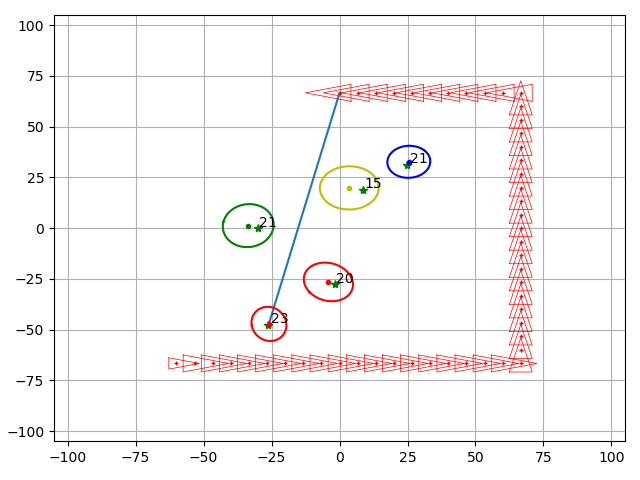
\includegraphics{5.png}
\end{figure}

    
    \begin{Verbatim}[commandchars=\\\{\}]
Iteration: 0
Estimated xEst:
[[-12.816]
 [-21.656]]
Estimated PEst:
[[65.917 -2.151]
 [-2.151 66.415]]
---------------------------------
Iteration: 5
Estimated xEst:
[[-12.816]
 [-21.656]
 [ 33.095]
 [ 35.514]
 [ 22.687]
 [ 16.831]
 [-40.615]
 [  3.564]]
Estimated PEst:
[[  65.917   -2.151    0.       0.       0.       0.       0.       0.   ]
 [  -2.151   66.415    0.       0.       0.       0.       0.       0.   ]
 [   0.       0.     184.872 -110.125    0.       0.       0.       0.   ]
 [   0.       0.    -110.125  164.333    0.       0.       0.       0.   ]
 [   0.       0.       0.       0.     134.436  -66.94     0.       0.   ]
 [   0.       0.       0.       0.     -66.94   127.617    0.       0.   ]
 [   0.       0.       0.       0.       0.       0.      24.156   -0.618]
 [   0.       0.       0.       0.       0.       0.      -0.618   21.502]]
---------------------------------
Iteration: 10
Estimated xEst:
[[-12.816]
 [-21.656]
 [ 33.095]
 [ 35.514]
 [ 10.433]
 [ 22.98 ]
 [-37.516]
 [  4.044]
 [-22.429]
 [-42.212]]
Estimated PEst:
[[  65.917   -2.151    0.       0.       0.       0.       0.       0.
     0.       0.   ]
 [  -2.151   66.415    0.       0.       0.       0.       0.       0.
     0.       0.   ]
 [   0.       0.     184.872 -110.125    0.       0.       0.       0.
     0.       0.   ]
 [   0.       0.    -110.125  164.333    0.       0.       0.       0.
     0.       0.   ]
 [   0.       0.       0.       0.      64.383  -26.848    0.       0.
     0.       0.   ]
 [   0.       0.       0.       0.     -26.848   54.432    0.       0.
     0.       0.   ]
 [   0.       0.       0.       0.       0.       0.      18.192   -0.372
     0.       0.   ]
 [   0.       0.       0.       0.       0.       0.      -0.372   16.094
     0.       0.   ]
 [   0.       0.       0.       0.       0.       0.       0.       0.
     8.597    5.833]
 [   0.       0.       0.       0.       0.       0.       0.       0.
     5.833   18.228]]
---------------------------------
Iteration: 15
Estimated xEst:
[[ -9.621]
 [-23.311]
 [ 22.587]
 [ 31.994]
 [ 10.433]
 [ 22.98 ]
 [-37.516]
 [  4.044]
 [-24.862]
 [-43.11 ]]
Estimated PEst:
[[ 21.331   1.436   0.      0.      0.      0.      0.      0.      0.
    0.   ]
 [  1.436  32.24    0.      0.      0.      0.      0.      0.      0.
    0.   ]
 [  0.      0.     53.354 -21.514   0.      0.      0.      0.      0.
    0.   ]
 [  0.      0.    -21.514  36.06    0.      0.      0.      0.      0.
    0.   ]
 [  0.      0.      0.      0.     64.383 -26.848   0.      0.      0.
    0.   ]
 [  0.      0.      0.      0.    -26.848  54.432   0.      0.      0.
    0.   ]
 [  0.      0.      0.      0.      0.      0.     18.192  -0.372   0.
    0.   ]
 [  0.      0.      0.      0.      0.      0.     -0.372  16.094   0.
    0.   ]
 [  0.      0.      0.      0.      0.      0.      0.      0.      2.791
    0.482]
 [  0.      0.      0.      0.      0.      0.      0.      0.      0.482
    8.928]]
---------------------------------
Iteration: 20
Estimated xEst:
[[ -9.621]
 [-23.311]
 [ 26.482]
 [ 30.962]
 [ 11.095]
 [ 19.45 ]
 [-37.485]
 [  3.069]
 [-25.135]
 [-43.887]]
Estimated PEst:
[[ 21.331   1.436   0.      0.      0.      0.      0.      0.      0.
    0.   ]
 [  1.436  32.24    0.      0.      0.      0.      0.      0.      0.
    0.   ]
 [  0.      0.     30.288  -8.93    0.      0.      0.      0.      0.
    0.   ]
 [  0.      0.     -8.93   17.702   0.      0.      0.      0.      0.
    0.   ]
 [  0.      0.      0.      0.     40.216 -11.223   0.      0.      0.
    0.   ]
 [  0.      0.      0.      0.    -11.223  29.051   0.      0.      0.
    0.   ]
 [  0.      0.      0.      0.      0.      0.     14.937   0.064   0.
    0.   ]
 [  0.      0.      0.      0.      0.      0.      0.064  12.972   0.
    0.   ]
 [  0.      0.      0.      0.      0.      0.      0.      0.      2.556
    0.048]
 [  0.      0.      0.      0.      0.      0.      0.      0.      0.048
    6.725]]
---------------------------------
Iteration: 25
Estimated xEst:
[[  0.145]
 [-24.146]
 [ 24.462]
 [ 33.171]
 [ 11.095]
 [ 19.45 ]
 [-37.485]
 [  3.069]
 [-25.603]
 [-44.457]]
Estimated PEst:
[[  7.212  -1.276   0.      0.      0.      0.      0.      0.      0.
    0.   ]
 [ -1.276  12.119   0.      0.      0.      0.      0.      0.      0.
    0.   ]
 [  0.      0.     24.466  -6.012   0.      0.      0.      0.      0.
    0.   ]
 [  0.      0.     -6.012  13.68    0.      0.      0.      0.      0.
    0.   ]
 [  0.      0.      0.      0.     40.216 -11.223   0.      0.      0.
    0.   ]
 [  0.      0.      0.      0.    -11.223  29.051   0.      0.      0.
    0.   ]
 [  0.      0.      0.      0.      0.      0.     14.937   0.064   0.
    0.   ]
 [  0.      0.      0.      0.      0.      0.      0.064  12.972   0.
    0.   ]
 [  0.      0.      0.      0.      0.      0.      0.      0.      2.439
   -0.042]
 [  0.      0.      0.      0.      0.      0.      0.      0.     -0.042
    5.712]]
---------------------------------
Iteration: 30
Estimated xEst:
[[  0.145]
 [-24.146]
 [ 24.462]
 [ 33.171]
 [ 10.973]
 [ 19.468]
 [-32.42 ]
 [  2.026]
 [-25.777]
 [-44.792]]
Estimated PEst:
[[ 7.212 -1.276  0.     0.     0.     0.     0.     0.     0.     0.   ]
 [-1.276 12.119  0.     0.     0.     0.     0.     0.     0.     0.   ]
 [ 0.     0.    24.466 -6.012  0.     0.     0.     0.     0.     0.   ]
 [ 0.     0.    -6.012 13.68   0.     0.     0.     0.     0.     0.   ]
 [ 0.     0.     0.     0.    28.354 -4.765  0.     0.     0.     0.   ]
 [ 0.     0.     0.     0.    -4.765 19.402  0.     0.     0.     0.   ]
 [ 0.     0.     0.     0.     0.     0.    11.286  0.976  0.     0.   ]
 [ 0.     0.     0.     0.     0.     0.     0.976 10.044  0.     0.   ]
 [ 0.     0.     0.     0.     0.     0.     0.     0.     2.26  -0.064]
 [ 0.     0.     0.     0.     0.     0.     0.     0.    -0.064  4.684]]
---------------------------------
Iteration: 35
Estimated xEst:
[[  0.39 ]
 [-24.429]
 [ 23.835]
 [ 33.531]
 [ 10.973]
 [ 19.468]
 [-32.451]
 [  1.909]
 [-25.788]
 [-45.652]]
Estimated PEst:
[[ 6.477 -0.936  0.     0.     0.     0.     0.     0.     0.     0.   ]
 [-0.936 10.237  0.     0.     0.     0.     0.     0.     0.     0.   ]
 [ 0.     0.    17.453 -2.488  0.     0.     0.     0.     0.     0.   ]
 [ 0.     0.    -2.488  9.266  0.     0.     0.     0.     0.     0.   ]
 [ 0.     0.     0.     0.    28.354 -4.765  0.     0.     0.     0.   ]
 [ 0.     0.     0.     0.    -4.765 19.402  0.     0.     0.     0.   ]
 [ 0.     0.     0.     0.     0.     0.    10.077  1.205  0.     0.   ]
 [ 0.     0.     0.     0.     0.     0.     1.205  9.155  0.     0.   ]
 [ 0.     0.     0.     0.     0.     0.     0.     0.     2.184 -0.053]
 [ 0.     0.     0.     0.     0.     0.     0.     0.    -0.053  4.393]]
---------------------------------
Iteration: 40
Estimated xEst:
[[ -2.554]
 [-24.196]
 [ 23.835]
 [ 33.531]
 [ 10.973]
 [ 19.468]
 [-32.451]
 [  1.909]
 [-26.124]
 [-45.974]]
Estimated PEst:
[[ 5.015e+00 -3.367e-01  0.000e+00  0.000e+00  0.000e+00  0.000e+00
   0.000e+00  0.000e+00  0.000e+00  0.000e+00]
 [-3.367e-01  7.264e+00  0.000e+00  0.000e+00  0.000e+00  0.000e+00
   0.000e+00  0.000e+00  0.000e+00  0.000e+00]
 [ 0.000e+00  0.000e+00  1.745e+01 -2.488e+00  0.000e+00  0.000e+00
   0.000e+00  0.000e+00  0.000e+00  0.000e+00]
 [ 0.000e+00  0.000e+00 -2.488e+00  9.266e+00  0.000e+00  0.000e+00
   0.000e+00  0.000e+00  0.000e+00  0.000e+00]
 [ 0.000e+00  0.000e+00  0.000e+00  0.000e+00  2.835e+01 -4.765e+00
   0.000e+00  0.000e+00  0.000e+00  0.000e+00]
 [ 0.000e+00  0.000e+00  0.000e+00  0.000e+00 -4.765e+00  1.940e+01
   0.000e+00  0.000e+00  0.000e+00  0.000e+00]
 [ 0.000e+00  0.000e+00  0.000e+00  0.000e+00  0.000e+00  0.000e+00
   1.008e+01  1.205e+00  0.000e+00  0.000e+00]
 [ 0.000e+00  0.000e+00  0.000e+00  0.000e+00  0.000e+00  0.000e+00
   1.205e+00  9.155e+00  0.000e+00  0.000e+00]
 [ 0.000e+00  0.000e+00  0.000e+00  0.000e+00  0.000e+00  0.000e+00
   0.000e+00  0.000e+00  2.047e+00 -1.720e-02]
 [ 0.000e+00  0.000e+00  0.000e+00  0.000e+00  0.000e+00  0.000e+00
   0.000e+00  0.000e+00 -1.720e-02  4.100e+00]]
---------------------------------
Iteration: 45
Estimated xEst:
[[ -2.554]
 [-24.196]
 [ 23.668]
 [ 32.254]
 [  8.694]
 [ 20.481]
 [-31.939]
 [  1.904]
 [-26.268]
 [-45.891]]
Estimated PEst:
[[ 5.015e+00 -3.367e-01  0.000e+00  0.000e+00  0.000e+00  0.000e+00
   0.000e+00  0.000e+00  0.000e+00  0.000e+00]
 [-3.367e-01  7.264e+00  0.000e+00  0.000e+00  0.000e+00  0.000e+00
   0.000e+00  0.000e+00  0.000e+00  0.000e+00]
 [ 0.000e+00  0.000e+00  1.490e+01 -1.492e+00  0.000e+00  0.000e+00
   0.000e+00  0.000e+00  0.000e+00  0.000e+00]
 [ 0.000e+00  0.000e+00 -1.492e+00  8.075e+00  0.000e+00  0.000e+00
   0.000e+00  0.000e+00  0.000e+00  0.000e+00]
 [ 0.000e+00  0.000e+00  0.000e+00  0.000e+00  2.140e+01 -1.664e+00
   0.000e+00  0.000e+00  0.000e+00  0.000e+00]
 [ 0.000e+00  0.000e+00  0.000e+00  0.000e+00 -1.664e+00  1.515e+01
   0.000e+00  0.000e+00  0.000e+00  0.000e+00]
 [ 0.000e+00  0.000e+00  0.000e+00  0.000e+00  0.000e+00  0.000e+00
   8.931e+00  1.303e+00  0.000e+00  0.000e+00]
 [ 0.000e+00  0.000e+00  0.000e+00  0.000e+00  0.000e+00  0.000e+00
   1.303e+00  8.634e+00  0.000e+00  0.000e+00]
 [ 0.000e+00  0.000e+00  0.000e+00  0.000e+00  0.000e+00  0.000e+00
   0.000e+00  0.000e+00  1.925e+00 -4.000e-03]
 [ 0.000e+00  0.000e+00  0.000e+00  0.000e+00  0.000e+00  0.000e+00
   0.000e+00  0.000e+00 -4.000e-03  3.854e+00]]
---------------------------------
Iteration: 50
Estimated xEst:
[[ -2.481]
 [-24.447]
 [ 24.457]
 [ 33.249]
 [  6.729]
 [ 20.721]
 [-32.23 ]
 [  2.238]
 [-26.312]
 [-46.758]]
Estimated PEst:
[[ 4.652e+00 -2.643e-01  0.000e+00  0.000e+00  0.000e+00  0.000e+00
   0.000e+00  0.000e+00  0.000e+00  0.000e+00]
 [-2.643e-01  6.625e+00  0.000e+00  0.000e+00  0.000e+00  0.000e+00
   0.000e+00  0.000e+00  0.000e+00  0.000e+00]
 [ 0.000e+00  0.000e+00  1.242e+01 -9.543e-01  0.000e+00  0.000e+00
   0.000e+00  0.000e+00  0.000e+00  0.000e+00]
 [ 0.000e+00  0.000e+00 -9.543e-01  7.189e+00  0.000e+00  0.000e+00
   0.000e+00  0.000e+00  0.000e+00  0.000e+00]
 [ 0.000e+00  0.000e+00  0.000e+00  0.000e+00  1.667e+01 -5.082e-01
   0.000e+00  0.000e+00  0.000e+00  0.000e+00]
 [ 0.000e+00  0.000e+00  0.000e+00  0.000e+00 -5.082e-01  1.261e+01
   0.000e+00  0.000e+00  0.000e+00  0.000e+00]
 [ 0.000e+00  0.000e+00  0.000e+00  0.000e+00  0.000e+00  0.000e+00
   7.952e+00  1.284e+00  0.000e+00  0.000e+00]
 [ 0.000e+00  0.000e+00  0.000e+00  0.000e+00  0.000e+00  0.000e+00
   1.284e+00  8.168e+00  0.000e+00  0.000e+00]
 [ 0.000e+00  0.000e+00  0.000e+00  0.000e+00  0.000e+00  0.000e+00
   0.000e+00  0.000e+00  1.869e+00 -7.258e-03]
 [ 0.000e+00  0.000e+00  0.000e+00  0.000e+00  0.000e+00  0.000e+00
   0.000e+00  0.000e+00 -7.258e-03  3.742e+00]]
---------------------------------
Iteration: 55
Estimated xEst:
[[ -2.481]
 [-24.447]
 [ 24.457]
 [ 33.249]
 [  3.411]
 [ 22.452]
 [-31.384]
 [  1.267]
 [-26.434]
 [-46.611]]
Estimated PEst:
[[ 4.652 -0.264  0.     0.     0.     0.     0.     0.     0.     0.   ]
 [-0.264  6.625  0.     0.     0.     0.     0.     0.     0.     0.   ]
 [ 0.     0.    12.419 -0.954  0.     0.     0.     0.     0.     0.   ]
 [ 0.     0.    -0.954  7.189  0.     0.     0.     0.     0.     0.   ]
 [ 0.     0.     0.     0.    13.435 -0.107  0.     0.     0.     0.   ]
 [ 0.     0.     0.     0.    -0.107 10.785  0.     0.     0.     0.   ]
 [ 0.     0.     0.     0.     0.     0.     5.875  1.027  0.     0.   ]
 [ 0.     0.     0.     0.     0.     0.     1.027  6.997  0.     0.   ]
 [ 0.     0.     0.     0.     0.     0.     0.     0.     1.818 -0.022]
 [ 0.     0.     0.     0.     0.     0.     0.     0.    -0.022  3.636]]
---------------------------------
Iteration: 60
Estimated xEst:
[[ -2.481]
 [-24.447]
 [ 24.109]
 [ 35.613]
 [  5.942]
 [ 21.308]
 [-33.057]
 [  0.546]
 [-26.368]
 [-46.962]]
Estimated PEst:
[[ 4.652 -0.264  0.     0.     0.     0.     0.     0.     0.     0.   ]
 [-0.264  6.625  0.     0.     0.     0.     0.     0.     0.     0.   ]
 [ 0.     0.    10.133 -0.95   0.     0.     0.     0.     0.     0.   ]
 [ 0.     0.    -0.95   6.246  0.     0.     0.     0.     0.     0.   ]
 [ 0.     0.     0.     0.    11.114 -0.052  0.     0.     0.     0.   ]
 [ 0.     0.     0.     0.    -0.052  9.286  0.     0.     0.     0.   ]
 [ 0.     0.     0.     0.     0.     0.     4.969  0.837  0.     0.   ]
 [ 0.     0.     0.     0.     0.     0.     0.837  6.371  0.     0.   ]
 [ 0.     0.     0.     0.     0.     0.     0.     0.     1.773 -0.041]
 [ 0.     0.     0.     0.     0.     0.     0.     0.    -0.041  3.535]]
---------------------------------
Iteration: 65
Estimated xEst:
[[ -3.124]
 [-23.662]
 [ 26.923]
 [ 33.303]
 [  6.745]
 [ 21.034]
 [-34.213]
 [ -0.489]
 [-26.368]
 [-46.962]]
Estimated PEst:
[[ 4.373 -0.301  0.     0.     0.     0.     0.     0.     0.     0.   ]
 [-0.301  6.161  0.     0.     0.     0.     0.     0.     0.     0.   ]
 [ 0.     0.     7.446 -0.928  0.     0.     0.     0.     0.     0.   ]
 [ 0.     0.    -0.928  4.761  0.     0.     0.     0.     0.     0.   ]
 [ 0.     0.     0.     0.     9.462 -0.065  0.     0.     0.     0.   ]
 [ 0.     0.     0.     0.    -0.065  8.015  0.     0.     0.     0.   ]
 [ 0.     0.     0.     0.     0.     0.     4.602  0.704  0.     0.   ]
 [ 0.     0.     0.     0.     0.     0.     0.704  6.085  0.     0.   ]
 [ 0.     0.     0.     0.     0.     0.     0.     0.     1.773 -0.041]
 [ 0.     0.     0.     0.     0.     0.     0.     0.    -0.041  3.535]]
---------------------------------
Iteration: 70
Estimated xEst:
[[ -2.136]
 [-23.708]
 [ 26.461]
 [ 33.374]
 [  2.48 ]
 [ 19.873]
 [-33.963]
 [  0.556]
 [-26.368]
 [-46.962]]
Estimated PEst:
[[ 4.139 -0.34   0.     0.     0.     0.     0.     0.     0.     0.   ]
 [-0.34   5.77   0.     0.     0.     0.     0.     0.     0.     0.   ]
 [ 0.     0.     6.643 -0.852  0.     0.     0.     0.     0.     0.   ]
 [ 0.     0.    -0.852  4.05   0.     0.     0.     0.     0.     0.   ]
 [ 0.     0.     0.     0.     7.297 -0.009  0.     0.     0.     0.   ]
 [ 0.     0.     0.     0.    -0.009  6.255  0.     0.     0.     0.   ]
 [ 0.     0.     0.     0.     0.     0.     4.296  0.553  0.     0.   ]
 [ 0.     0.     0.     0.     0.     0.     0.553  5.809  0.     0.   ]
 [ 0.     0.     0.     0.     0.     0.     0.     0.     1.773 -0.041]
 [ 0.     0.     0.     0.     0.     0.     0.     0.    -0.041  3.535]]
---------------------------------
Iteration: 75
Estimated xEst:
[[ -2.405]
 [-24.287]
 [ 26.461]
 [ 33.374]
 [  2.532]
 [ 19.512]
 [-33.883]
 [  0.88 ]
 [-26.099]
 [-46.648]]
Estimated PEst:
[[ 3.973 -0.403  0.     0.     0.     0.     0.     0.     0.     0.   ]
 [-0.403  5.429  0.     0.     0.     0.     0.     0.     0.     0.   ]
 [ 0.     0.     6.643 -0.852  0.     0.     0.     0.     0.     0.   ]
 [ 0.     0.    -0.852  4.05   0.     0.     0.     0.     0.     0.   ]
 [ 0.     0.     0.     0.     5.968 -0.055  0.     0.     0.     0.   ]
 [ 0.     0.     0.     0.    -0.055  5.322  0.     0.     0.     0.   ]
 [ 0.     0.     0.     0.     0.     0.     4.033  0.424  0.     0.   ]
 [ 0.     0.     0.     0.     0.     0.     0.424  5.559  0.     0.   ]
 [ 0.     0.     0.     0.     0.     0.     0.     0.     1.744 -0.074]
 [ 0.     0.     0.     0.     0.     0.     0.     0.    -0.074  3.419]]
---------------------------------
Iteration: 80
Estimated xEst:
[[ -2.642]
 [-26.388]
 [ 25.704]
 [ 33.418]
 [  2.532]
 [ 19.512]
 [-33.883]
 [  0.88 ]
 [-26.082]
 [-46.904]]
Estimated PEst:
[[ 3.73  -0.514  0.     0.     0.     0.     0.     0.     0.     0.   ]
 [-0.514  4.855  0.     0.     0.     0.     0.     0.     0.     0.   ]
 [ 0.     0.     5.784 -0.563  0.     0.     0.     0.     0.     0.   ]
 [ 0.     0.    -0.563  3.682  0.     0.     0.     0.     0.     0.   ]
 [ 0.     0.     0.     0.     5.968 -0.055  0.     0.     0.     0.   ]
 [ 0.     0.     0.     0.    -0.055  5.322  0.     0.     0.     0.   ]
 [ 0.     0.     0.     0.     0.     0.     4.033  0.424  0.     0.   ]
 [ 0.     0.     0.     0.     0.     0.     0.424  5.559  0.     0.   ]
 [ 0.     0.     0.     0.     0.     0.     0.     0.     1.697 -0.133]
 [ 0.     0.     0.     0.     0.     0.     0.     0.    -0.133  3.201]]
---------------------------------
Iteration: 85
Estimated xEst:
[[ -2.642]
 [-26.388]
 [ 26.464]
 [ 33.621]
 [  2.532]
 [ 19.512]
 [-33.883]
 [  0.88 ]
 [-26.162]
 [-46.83 ]]
Estimated PEst:
[[ 3.73  -0.514  0.     0.     0.     0.     0.     0.     0.     0.   ]
 [-0.514  4.855  0.     0.     0.     0.     0.     0.     0.     0.   ]
 [ 0.     0.     3.552  0.095  0.     0.     0.     0.     0.     0.   ]
 [ 0.     0.     0.095  2.709  0.     0.     0.     0.     0.     0.   ]
 [ 0.     0.     0.     0.     5.968 -0.055  0.     0.     0.     0.   ]
 [ 0.     0.     0.     0.    -0.055  5.322  0.     0.     0.     0.   ]
 [ 0.     0.     0.     0.     0.     0.     4.033  0.424  0.     0.   ]
 [ 0.     0.     0.     0.     0.     0.     0.424  5.559  0.     0.   ]
 [ 0.     0.     0.     0.     0.     0.     0.     0.     1.679 -0.155]
 [ 0.     0.     0.     0.     0.     0.     0.     0.    -0.155  3.086]]
---------------------------------
Iteration: 90
Estimated xEst:
[[ -3.567]
 [-26.89 ]
 [ 25.565]
 [ 33.097]
 [  2.588]
 [ 19.468]
 [-33.883]
 [  0.88 ]
 [-26.162]
 [-46.83 ]]
Estimated PEst:
[[ 3.45  -0.53   0.     0.     0.     0.     0.     0.     0.     0.   ]
 [-0.53   4.054  0.     0.     0.     0.     0.     0.     0.     0.   ]
 [ 0.     0.     2.929  0.111  0.     0.     0.     0.     0.     0.   ]
 [ 0.     0.     0.111  2.597  0.     0.     0.     0.     0.     0.   ]
 [ 0.     0.     0.     0.     5.432 -0.025  0.     0.     0.     0.   ]
 [ 0.     0.     0.     0.    -0.025  4.897  0.     0.     0.     0.   ]
 [ 0.     0.     0.     0.     0.     0.     4.033  0.424  0.     0.   ]
 [ 0.     0.     0.     0.     0.     0.     0.424  5.559  0.     0.   ]
 [ 0.     0.     0.     0.     0.     0.     0.     0.     1.679 -0.155]
 [ 0.     0.     0.     0.     0.     0.     0.     0.    -0.155  3.086]]
---------------------------------
Iteration: 95
Estimated xEst:
[[ -4.215]
 [-27.019]
 [ 25.475]
 [ 32.677]
 [  2.588]
 [ 19.468]
 [-33.224]
 [  1.156]
 [-26.094]
 [-46.799]]
Estimated PEst:
[[ 3.365 -0.52   0.     0.     0.     0.     0.     0.     0.     0.   ]
 [-0.52   3.833  0.     0.     0.     0.     0.     0.     0.     0.   ]
 [ 0.     0.     2.496  0.073  0.     0.     0.     0.     0.     0.   ]
 [ 0.     0.     0.073  2.493  0.     0.     0.     0.     0.     0.   ]
 [ 0.     0.     0.     0.     5.432 -0.025  0.     0.     0.     0.   ]
 [ 0.     0.     0.     0.    -0.025  4.897  0.     0.     0.     0.   ]
 [ 0.     0.     0.     0.     0.     0.     3.665  0.235  0.     0.   ]
 [ 0.     0.     0.     0.     0.     0.     0.235  4.818  0.     0.   ]
 [ 0.     0.     0.     0.     0.     0.     0.     0.     1.664 -0.165]
 [ 0.     0.     0.     0.     0.     0.     0.     0.    -0.165  2.959]]
---------------------------------
    \end{Verbatim}

    \begin{center}
    \adjustimage{max size={0.9\linewidth}{0.9\paperheight}}{output_36_3.png}
    \end{center}
    { \hspace*{\fill} \\}
    
    \begin{center}
    \adjustimage{max size={0.9\linewidth}{0.9\paperheight}}{output_36_4.png}
    \end{center}
    { \hspace*{\fill} \\}
    
    \hypertarget{thinking-about-it-2}{%
\subsubsection{Thinking about it (2)}\label{thinking-about-it-2}}

Having taken a look at the logger and its output, you will be able to
\textbf{answer the following questions}:

\begin{itemize}
\item
  What information is shown in the figures produced by the logger?

  The logarithm of the determinant of covariance matrices and the
  logarithm of the error with respect the time
\item
  The information about the error and the determinant of the covariance
  is provided for first time at different iterations of the algorithm
  for each landmark. Is that an error? Why is this happening?

  No.~This happens because we only measure one distance to one landmark
  in one instance of time. Therefore, the first one we measure will fall
  down before the last one we measure
\item
  The error associated to each landmark not always decreases with new
  observations. Why could this happen?

  Because of the uncertainty of the sensor, it could happen that we may
  drift away from the expected position of the landmark.
\item
  On the contrary, the determinant of the covariance matrix associated
  to each landmark always decreases when new observations are available.
  Is this an error? Why?

  No.~This happens because the more measures I have of something, the
  less uncertainty I have. Therefore, by having more measurements and
  reducing uncertainty, the value of the determinant of the covariance
  matrix goes down.
\end{itemize}


    % Add a bibliography block to the postdoc
    
    
    
\end{document}
